\documentclass[reprint,superscriptaddress,prb,showkeys]{revtex4-2}
\usepackage{empheq}
\usepackage{float}
\usepackage{lipsum}
\usepackage{mathtools, cuted}
\usepackage{esvect}
\usepackage{xcolor}
\usepackage[caption = false]{subfig}
\usepackage{graphicx}
\usepackage{dcolumn}
\usepackage{bm}
\usepackage{hyperref}
\usepackage{physics}
\usepackage[mathlines]{lineno}
\usepackage[capitalise]{cleveref}
\usepackage[english]{babel}
\usepackage{orcidlink}
% \usepackage{natbib}
\usepackage{amsmath}
\usepackage{amssymb}

\usepackage{listings}

\lstset{
    basicstyle=\ttfamily\small,
    keywordstyle=\color{blue},
    commentstyle=\color{gray},
    columns=fullflexible,
    frame=single,
    breaklines=true,
    captionpos=b,
    numbers=left,
    numberstyle=\tiny\color{gray},
    escapeinside={(*@}{@*)}
}
\usepackage{algorithm}
\usepackage{algpseudocode}

%------------- COMMANDS -------------

\newcommand{\C}{\mathbb{C}} %complex
\newcommand{\R}{\mathbb{R}} %reals
\newcommand{\Z}{\mathbb{Z}} %integers
\renewcommand{\P}{\mathbb{P}} %prob

\newcommand{\m}{\text{m}} %m index
\newcommand{\M}{\text{M}} %m index
\newcommand{\N}{\text{N}} %n index
\newcommand{\n}{\text{n}} %n index
\renewcommand{\a}{\textbf{\text{a}}} %a index

\newcommand{\brac}[1]{\left(#1 \right)} %nice brackets
\newcommand{\bk}[1]{\langle #1 \rangle} 

\newcommand{\TODO}[1]{\textcolor{red}{TODO: #1}}


%------------- MAIN -------------

\begin{document}

\title{Multistimulus Machine Learning in Microfluidic Memristor Networks}

\author{Monica Conte}
\affiliation{Soft Condensed Matter \& Biophysics, Debye Institute for Nanomaterials Science, Utrecht University, Princetonplein 1, 3584 CC Utrecht, The Netherlands,}
\author{René van Roij}
\affiliation{Institute for Theoretical Physics, Utrecht University, Princetonplein 5, 3584 CC Utrecht, The Netherlands.}
\author{Marjolein Dijkstra}
\affiliation{Soft Condensed Matter \& Biophysics, Debye Institute for Nanomaterials Science, Utrecht University, Princetonplein 1, 3584 CC Utrecht, The Netherlands,}

\date{\today}

\begin{abstract}
Inspired by the brain's energy-efficient processing, we propose a physical implementation of artificial neural networks to surpass digital systems in thier capabilities. We consider a network with nodes connected by conical microfluidic memristor channels filled with aqueous electrolyte [1]. These memristive channels exhibit tunable conductance, in response to electrical, chemical, and mechanical stimuli, as well as to changes in channel geometry. Leveraging this multistimulus adaptability, we develop a hybrid training algorithm that treats either the channel geometry or external stimuli as adjustable weights. In this framework, the system itself performs the feedforward pass through physical relaxation, while a combined physical-numerical gradient descent executes the backward pass. The network performs basic learning tasks, such as input-output voltage mapping and linear regression with bias.
\end{abstract}
\maketitle

\renewcommand{\figurename}{FIG.}

\section{\label{sec:Intro}Introduction}

% ## Artificial Neural Networks ##
% - What they can achieve
% - Energy cost
% - Explain the two phases

Modern computing algorithms are able to efficiently perform complicated numerical and symbolic operations, but their sequential structure limits their performance on more perceptual tasks. Inspired by the architecture and the functioning of the human brain, that performs tasks via distributed and parallel fashion, artificial neural network (ANN) algorithms outreached traditional computing achieving remarkable success in challenging tasks, such as visual and audio pattern recognition~\cite{pattern_recognition,review_image_rec, speech_rec} to natural language processing and became central to many technological advancements in the field of artificial intelligence\cite{ai_tech1}.

Recent developments in artificial intelligence have been driven by the computational power of Graphics Processing Units and the availability of large amounts of data. However, as ANNs continue to grow in size and complexity, their energy demands have increased substantially, ultimately impacting their efficiency and limiting their scalability \cite{energy_cost_ml1, energy_cost_ml2}. Meanwhile, the gap between the accelerating computational needs of AI training and the gradual improvements in traditional silicon-based hardware, as historically described by Moore’s Law, has highlighted the need for innovative computing architectures. One promising alternative is the development of physical neural networks (PNNs), which train physical processes rather than relying solely on digital calculations \cite{trainingphysicalneuralnetworks,backporp_pnn}. Because physical systems can often achieve faster and more energy-efficient operations than their digital representations, this direction constitutes a promising research direction to address this issue.

Applications of PNNs have been explored across diverse fields, including optics \cite{optics1}, electronics \cite{electronics1}, photonics \cite{acoustic1} and mechanical systems \cite{mechanics1}, among others. Many existing training algorithms rely entirely on in silico methods, which often face challenges when transferring the learned model to real physical devices. To address this, hybrid training approaches have been proposed, where the inference phase is executed physically while the backward phase is computed numerically\cite{backporp_pnn}. Other methods, based on coupled learning\cite{supervised_learning}, implement local learning rules at the level of each connection or edge\cite{demonstr_coupled_learning}. Applying local rules removed the need of the optimiziation of a global cost function during learning, as in standard backpropagation methods. However, these approaches still face the need for two identical physical systems to apply different boundary conditions. In this work, we propose a novel algorithm in which both inference and backpropagation are carried out mainly taking advantage of the physical processes inherent in the system, specifically leveraging the natural relaxation dynamics of the system in response to external stimuli and weight modifications.

A key advantage of PNNs is their ability to more closely emulate certain functional aspects of biological neural systems. One of the defining features of the brain is its capacity to process and integrate multiple types of stimuli, such as electrical, chemical, and mechanical inputs, simultaneously. This multimodal responsiveness is believed to contribute significantly to the brain’s efficiency and adaptability \cite{}. Inspired by this functionality, we base our approach on physical neural networks constructed from memristive elements. Specifically, we utilize ionic microfluidic channels in aqueous solutions\cite{Rene_IonicNeuromorphic}, which exhibit the ability to respond concurrently to diverse physical stimuli. This characteristic is central to the operation of our proposed training algorithm.

% ## What we could achive ##

% ## Structure of the paper ##

The paper is organized as follows. \cref{sec:memristor_network} presents the physical network we define using memristor elements, called memristor network, and explains how this system is numerically solved. \cref{sec:training} describes the training algorithm that we use to achieve desired responses of the memristor network. In \cref{sec:train_memr_vd}, we exemplify the proposed algorithm by training a simple system, namely a voltage divider, for input-output voltage mapping. \cref{sec:train_memr_nw} shows a bigger network able to be trained for more complex input-output relationships. Finally, in \cref{sec:linear_regression} we adapt the training algorthm to train a network to perform a linear regression with bias. This section is followed by conclusions and suggestions for future work in \cref{sec:concl}.
% \newpage

\section{\label{sec:memristor_network}Memristor Network}

The PNN we consider is an electrical network made of nodes connected by resistive elements. As resistive elements, we consider conical microfluidic channels, schematically represented in \cref{fig:memristor_scheme}. 
\begin{figure}[h]
    \centering
    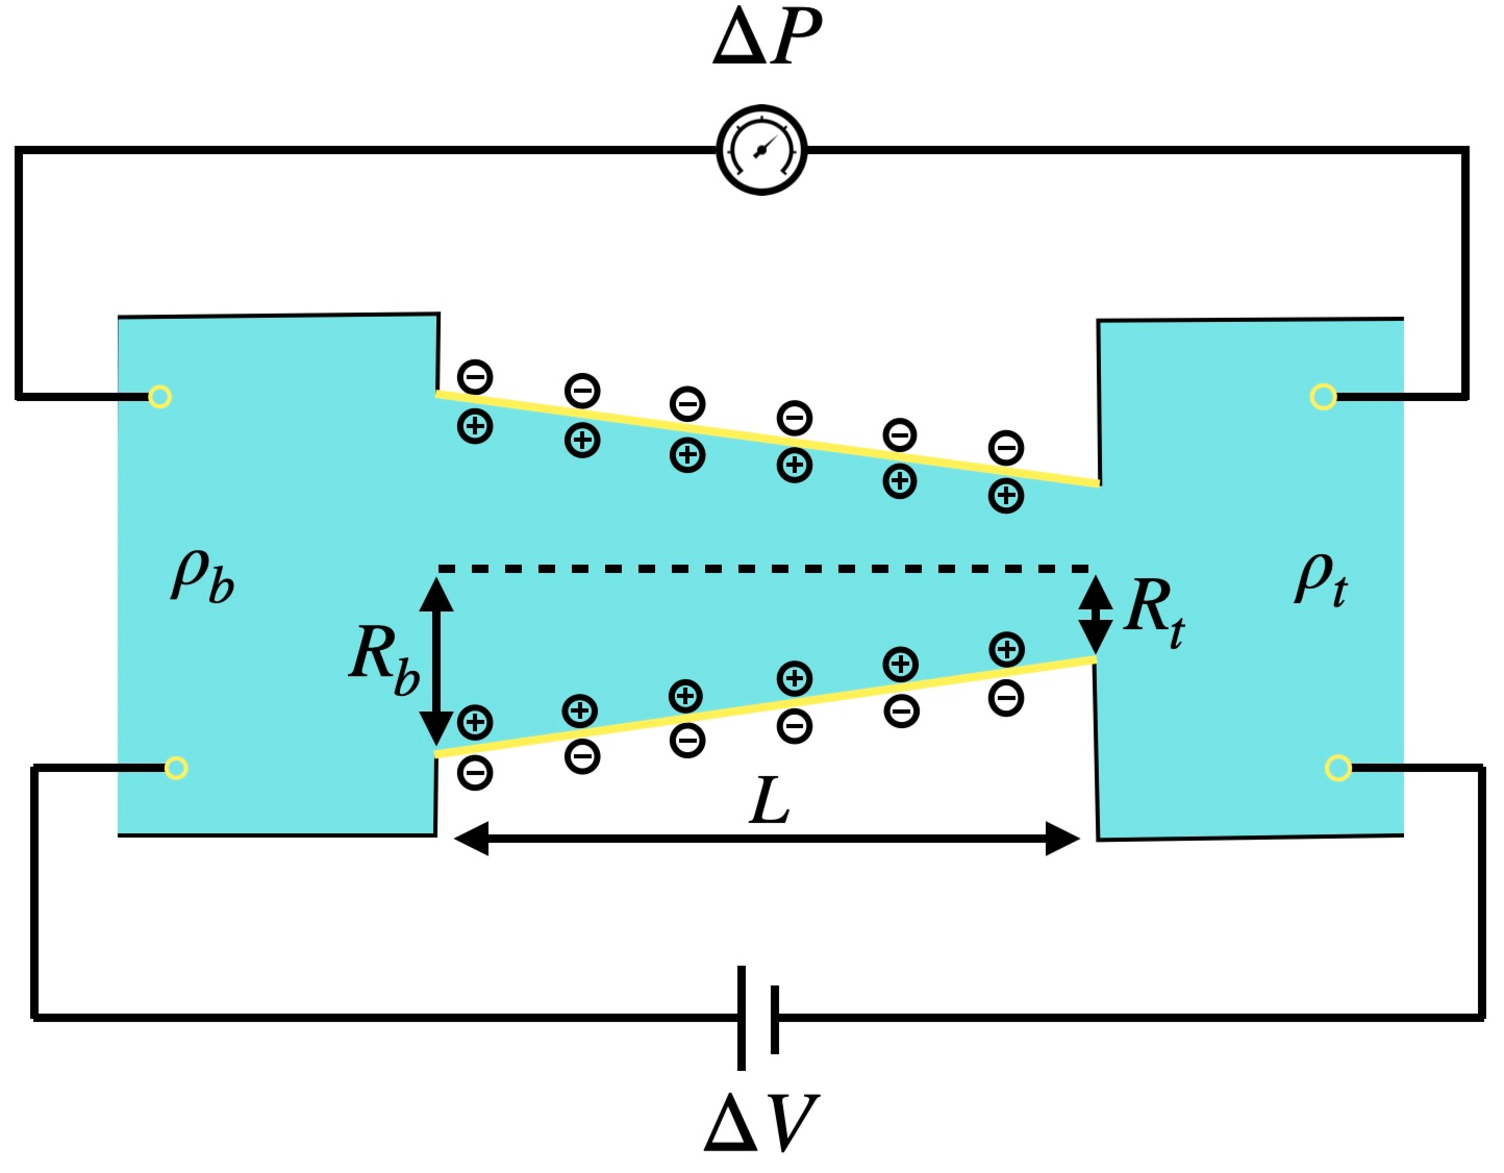
\includegraphics[width=\columnwidth]{plots/memristor/memristor_scheme.pdf}
    \caption{A schematic representation of the conical fluidic memristor. A cone of length $L$, base radius $R_b$ and tip radius $R_t$ with charged surface connects two bulk reservoirs of a 1:1 electrolyte in an aqueous solution. The bulk density in the base $\rho_b$ differs from the bulk density in the tip $\rho_t$. At the far side of the memristor, an electrical potential and pressure drop are applied. Overall, this results in a chemical, electrical and mechanical sensitive system.}\label{fig:memristor_scheme}
\end{figure} 
An azimuthally symmetric conical channel connects two reservoirs that contain an incompressible aqueous 1:1 electrolyte with viscosity $\eta=1.0$1mPa s and electric permittivity $\epsilon = 0.71$nF$\text{m}^{-1}$ containing ions with diffusion coefficient $D = 1.75\mu \text{m}^2 \text{ms}^{-1}$ and charge $\pm e$, with $e$ the proton charge. The cone has a base radius of $R_b = 200$nm, a tip radius of $R_t=50$nm and has length $L = 10\mu$m, which sets it in the long channel limit, where entrance and exit effects can be neglected. The walls of the channel are homogeneously charged and generate a surface potential $\psi_0$ that attracts the opposite-sign ions present in the solution due to the dissociation of the electrolyte. The electric potential decreases exponentially away from the surface due to the electrostatic screening of the attracted ions: an electric double layer (EDL) forms on the charged surfaces. 

At the far side of both reservoirs, electrical potential, pressure and ion concentration are imposed. As a result, the memristor feels a potential drop $\Delta V = V_b - V_t$ defined as the difference between the potential in the base and in the tip. The ions within the EDL region generate an electro-osmotic fluid flow $Q_V = (\pi R_b R_t\epsilon\psi_0/L\eta)\Delta V$. Meanwhile, the pressure drop $\Delta P = P_b - P_t$, given by the difference between the base and the tip pressure, induces a Poiseuille-like flow $Q_P = (\pi R_b^3 R_t^3/8L\eta\langle R^2\rangle)\Delta P$. Finally, the ions experience a salt concentration gradient $\Delta \rho = \rho_b - \rho_t$, defined by the difference between the ion concentration in the reservoir connected to the base of the channel, $\rho_b$, and the concentration in the reservoir connected to the tip, $\rho_t$. Consequently, a diffusive fluid flow arises. However, we consider only the pressure and potential contributions to the total fluid flow, $Q = Q_P + Q_V$, assuming the diffusive flow to be negligible.  The resulting fluid flow generates non-trivial ion concentration profiles which, in turn, directly influence the channel's conductance $g$. 
%It has already been shown that, for $\Delta P = 0$, the channel shows current rectification, thus working as a diode \cite{}, due to concentration polarization.  

In the steady-state, the channel is exposed to constant chemical, pressure and electrical signal, the corresponding conductance $g_{\infty}\brac{\boldsymbol{\Delta}}$ depends on the three stimuli $\boldsymbol{\Delta}= (\Delta V, \Delta P, \Delta \rho)$ and is determined by the ion concentration profiles according to 
\[
\frac{g_{\infty}\brac{\boldsymbol{\Delta}}}{g_0} = \int_0^{L} \frac{\bar{\rho}\left(x, \boldsymbol{\Delta}\right)}{2\rho_b L} dx                                           
\]
where $g_0$ is the Ohmic conductance and $\bar{\rho}(x)$ the radially averaged salt concentration as a function of $x\in[0,L]$\cite{Rene_IonicNeuromorphic}. By solving the stationary condition of the total salt flux, an expression for the average salt concentration can be found and reads
\begin{multline}
\frac{\bar{\rho}\left(x, \boldsymbol{\Delta}\right)}{2\rho_b} = 1 - \frac{\Delta \rho}{\rho_b} \mathcal{I}\left(x, \Delta V, \Delta P\right) \\
 + \frac{ \rho_{in}\left( \Delta V \right) }{2\rho_b \text{Pe}} \left[ \mathcal{F}(x) - \mathcal{I}\left(x, \Delta V, \Delta P\right) \right]
\label{eq:rho_average}
\end{multline}
where we defined, for the sake of simplicity and readability, two functions
\[
\mathcal{I}\left(x, \Delta V, \Delta P\right) = \frac{e^{\frac{x}{L}\frac{R_t^2}{R_b R(x)} \text{Pe}}-1}{e^{\frac{R_t}{R_b} \text{Pe}}-1}, \ \ \ \ \mathcal{F}(x) = \frac{x}{L}\frac{R_t}{R(x)}.
\]
Moreover, we introduced an expression for the concentration inhomogeneity 
\[
\rho_{in}\brac{\Delta V} = 2\frac{(R_b-R_t)\sigma}{R_t^2}\frac{e\Delta V}{k_B T}
\]
and the Péclet number
$
\text{Pe} = QL/D\pi R_t^2
$
which quantifies the importance of the flow $Q$ over diffusion \cite{Rene_PressureSensitive}.

%To better deal with numerical instabilities, we use a limit expression of \cref{eq:rho_average} when $\text{Pe} \ll \left( R_b/R_t \right)^2$ \cite{Rene_PressureSensitive}. With this consideration, the expression for the average salt concentration we use is the following
%\[
%\frac{\rho(x)}{2\rho_b} = 
%\begin{array}{cc}
 % \{ & 
  %  \begin{array}{cc}
   %   0 & x\leq 0 \\
    %  \frac{100-x}{100} & 0\leq x\leq 100
    %\end{array}
%\end{array}
%\]

When the external stimuli vary dynamically in time, they generate ion accumulation and depletion in the channel, changing consequently the conductivity. We assume the dynamics of the time-dependent conductance $g(t)$ as a single exponential decay towards the steady-state conductance $g_{\infty}$ with a diffusion-like timescale $\tau = L^2/12D$, as in Ref. \cite{Rene_IonicNeuromorphic}. The equation for the conductance reads
\begin{equation}
\frac{\partial g\brac{\boldsymbol{\Delta}(t), t}}{\partial t} = \frac{g_{\infty}\brac{\boldsymbol{\Delta}(t)}-g\brac{\boldsymbol{\Delta}(t), t}}{\tau}
\label{eq:eqofmotconductance}
\end{equation}
with $\boldsymbol{\Delta}(t) = \brac{\Delta V\brac{t},\Delta P\brac{t}, \Delta \rho\brac{t}}$.
As in Ref. \cite{Rene_IonicNeuromorphic}, we consider the time scale relative to voltage-driven ion accumulation or depletion in the channel. We justify this choice by stating that pressure-driven dynamics is faster and recalling that we neglect chemically-driven transport. Due to the fact that the conductance depends on the history of the signals applied, this system is called memristor. Aside from the direct dependence of the conductance on external stimuli, there is also an implicit dependence on geometrical properties, such as length $L$ and base radius $R_b$, that we address in this work.

The PNN is composed of $N$ nodes, an example is shown in \cref{fig:memristor_network}. 
\begin{figure}[t]
    \centering
    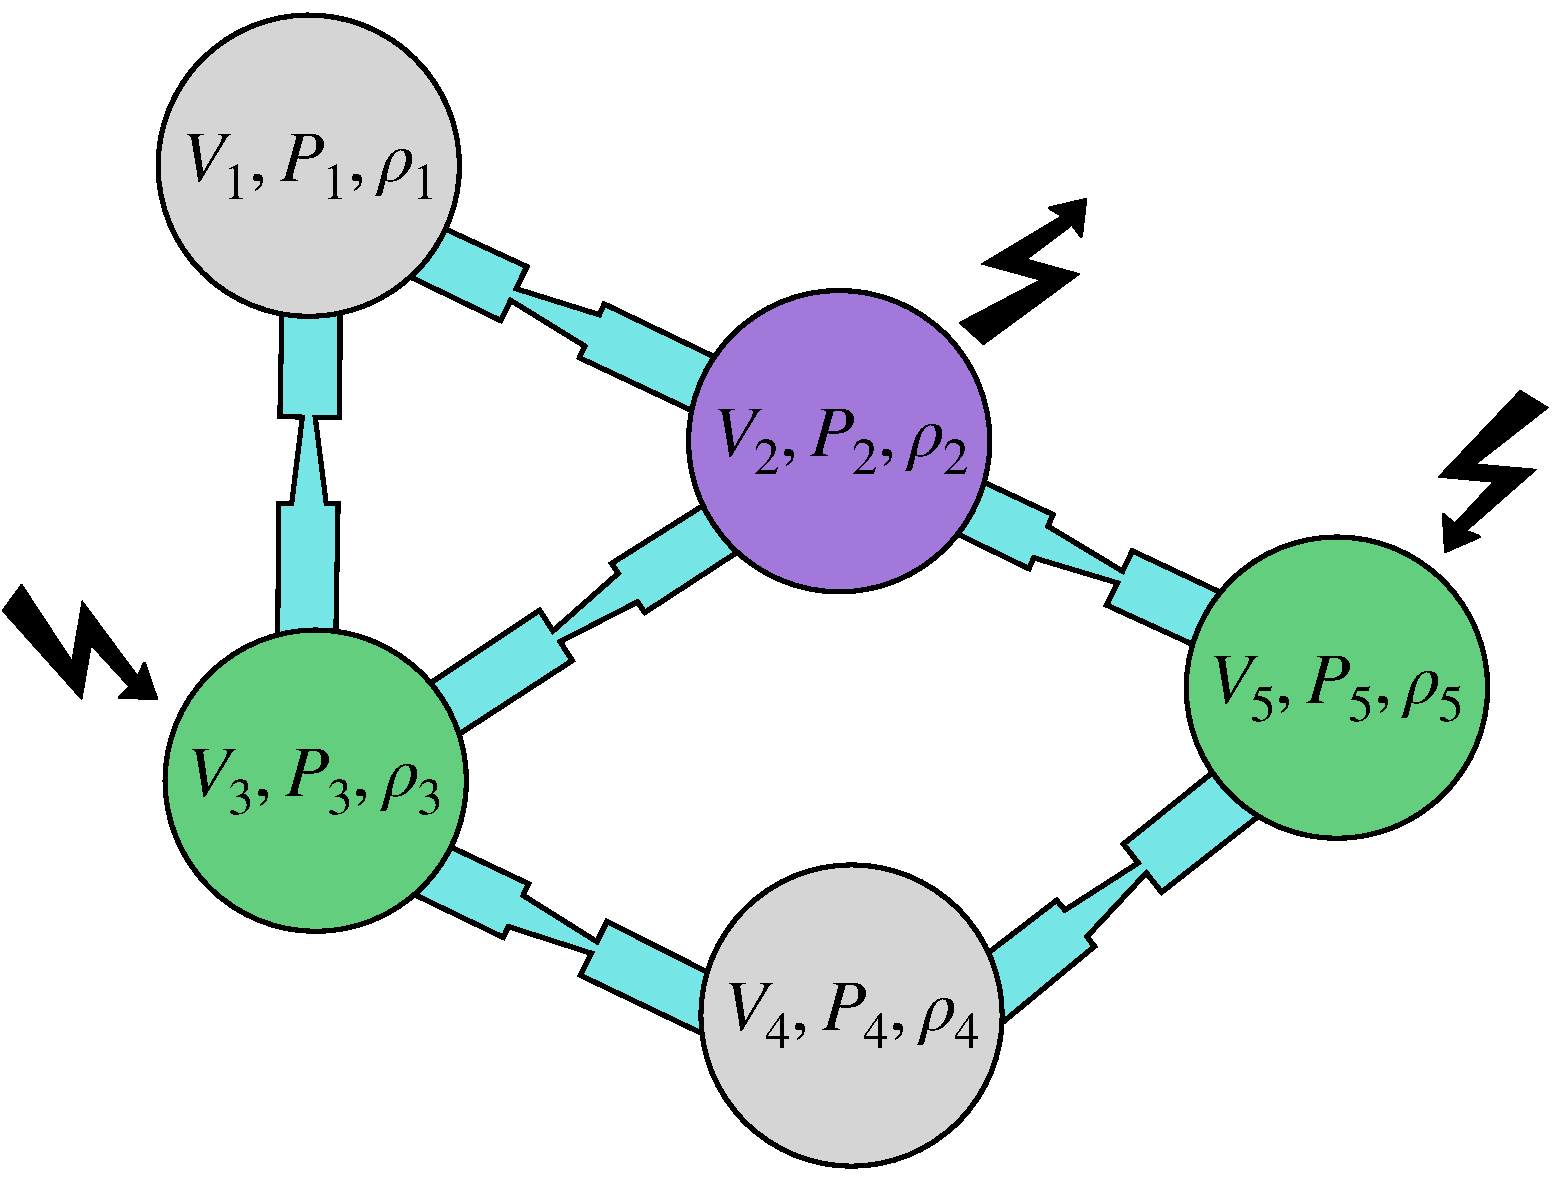
\includegraphics[width=0.6\columnwidth]{plots/memristor/memristor_network.pdf}
    \caption{An example of a network of five nodes connected by six memristors. The nodes are divided in input nodes (green circles), hidden nodes (grey nodes) and output nodes (purple circles) each of them is characterized by a triplet of physical quantities, representing the potential, pressure, and density. Th resulting stimuli on the memristor is given by the difference between base and tip signal, it thus depends on the orientation of the memristor. In the case of the memristor that connects the first and the second node, for example, the external stimuli are $\Delta V = V_2 - V_1$, $\Delta P = P_2 - P_1$ and $\Delta \rho = \rho_2 - \rho_1$. The zig-zag lines directed towards the input nodes indicate where the electrical signal is applied, while the zig-zag lines pointing outwards from the nodes indicate where the electrical signal is measured.}
    \label{fig:memristor_network}
\end{figure} 
Each node $\n\in[1,N]$ is characterized by a value of electrical potential $V_{\n}$, pressure $P_{\n}$ and bulk density $\rho_{\n}$. Even though each node in the network is characterized by three physical properties, only electrical current flows through the network. This current propagates via the memristive elements, enabling modifications to the electric potential at other nodes. In contrast, pressure and density are externally imposed at each node and do not propagate through the network. The set of nodes is divided in three sets. A node belongs to the set of \textit{input nodes} if it is used to input current in the circuit, its value of voltage is known and fixed. After the inputs are imposed, the electrical signal travels through the network and the resulting output potential is read in the nodes belonging to \textit{output nodes}. The remaining nodes, that do not function as input or output, are included in the set of \textit{hidden nodes}.

The nodes in the PNN are connected by $M$ memristive elements. Consequently, a memristor connecting two nodes experiences a potential drop, pressure drop and concentration gradient given by the difference between the node where the base of the memristor is connected to, and the node to which the tip is linked. The memristor is characterized by its conductance state $g_{\m}$ with $\m\in[1,M]$, consequence of both the geometry parameters and the external stimuli.
To solve numerically the resulting circuit, it is necessary to simultaneously address the circuit equations and the time evolution equation for the memristors' conductance. 
The circuit equations are handled using the open-source circuit solver \textsc{AHKAB}\cite{}, which computes the electric potentials at the nodes and the currents through the edges discretizing the differential equations in timesteps $\Delta t$. To incorporate the memristive elements, we approximate the time evolution of the conductances using a discretized form of \cref{eq:eqofmotconductance}, employing the Euler-forward method. Specifically, the conductance at a given time-step is calculated from its value at the previous time-step as:
\begin{multline}
    g_{\m}\brac{\boldsymbol{\Delta}(t), t} = g_{\m}\brac{\boldsymbol{\Delta}(t), t-\Delta t} + \\
    \frac{g_{\m,\infty}\brac{\boldsymbol{\Delta}(t)-g_{\m}\brac{\boldsymbol{\Delta}, t}}}{\tau}\Delta t.
\end{multline}
In this work, we only apply constant voltage supplies to the input nodes of the circuit. Nonetheless, we notice that solving the dynamical equations is needed due to the dynamical change in the conductance of the memristors that, in turn, results in time-dependent potential drops across them. A more detailed illustration of the algorithm that solves the circuit, along with an analysis of the relaxation to the steady state of the memristor network, is provided in \cref{app:dyn_evol_steady_state}.

\section{\label{sec:training}Training Algorithm for a Memristor Network}
\begin{figure}[b]
    \centering
    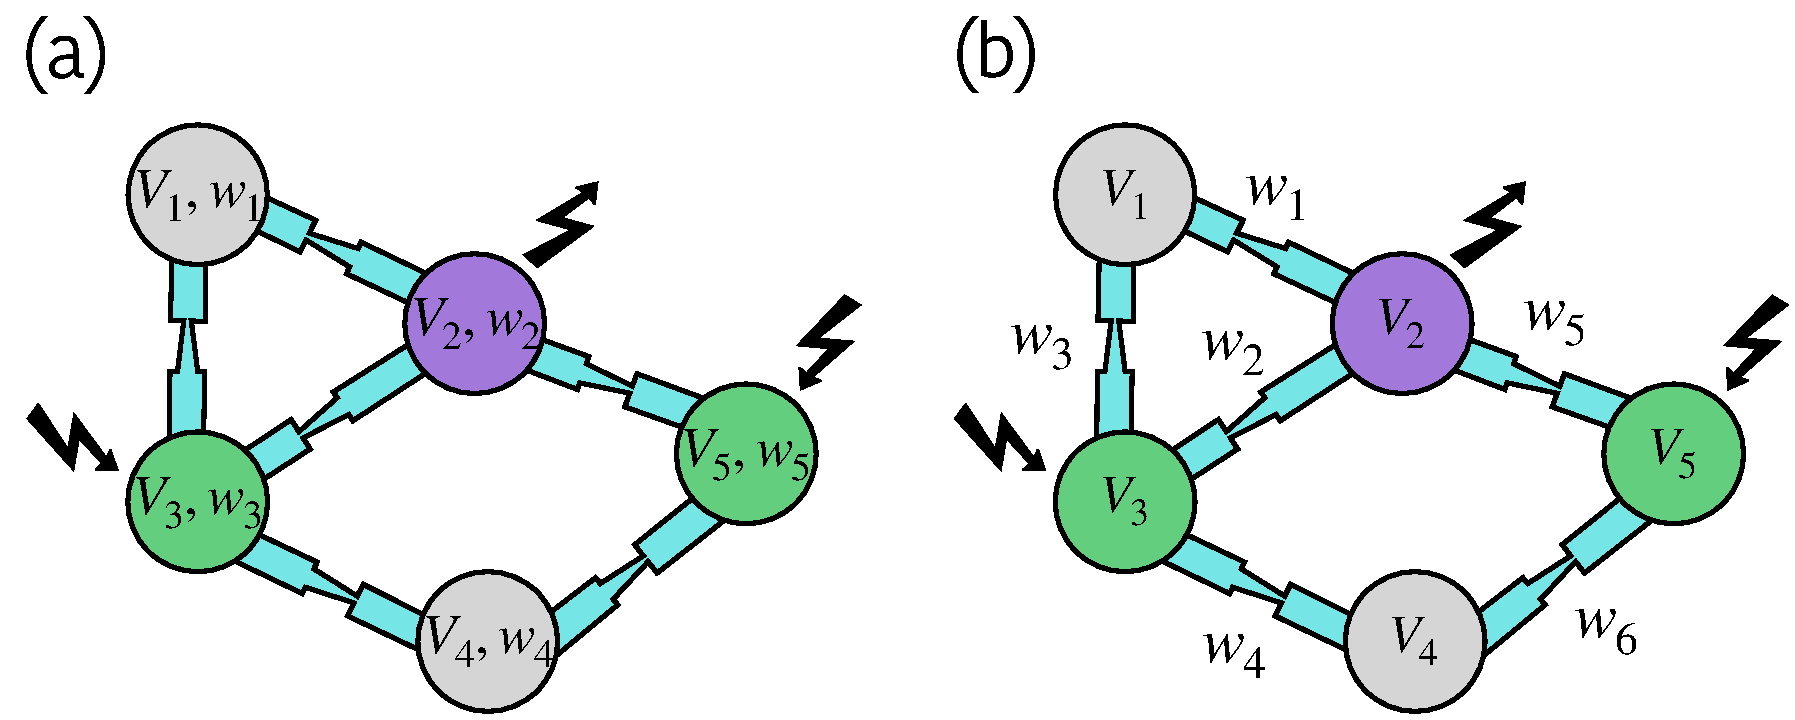
\includegraphics[width=0.8\columnwidth]{plots/training/two_types_weights.pdf}
    \caption{(a) Memristor network with weights defined in the nodes. (b) Memristor network where wegiths characterize each edge.}
    \label{fig:two_types_weights}
\end{figure} 
\begin{figure*}[t] 
    \centering
    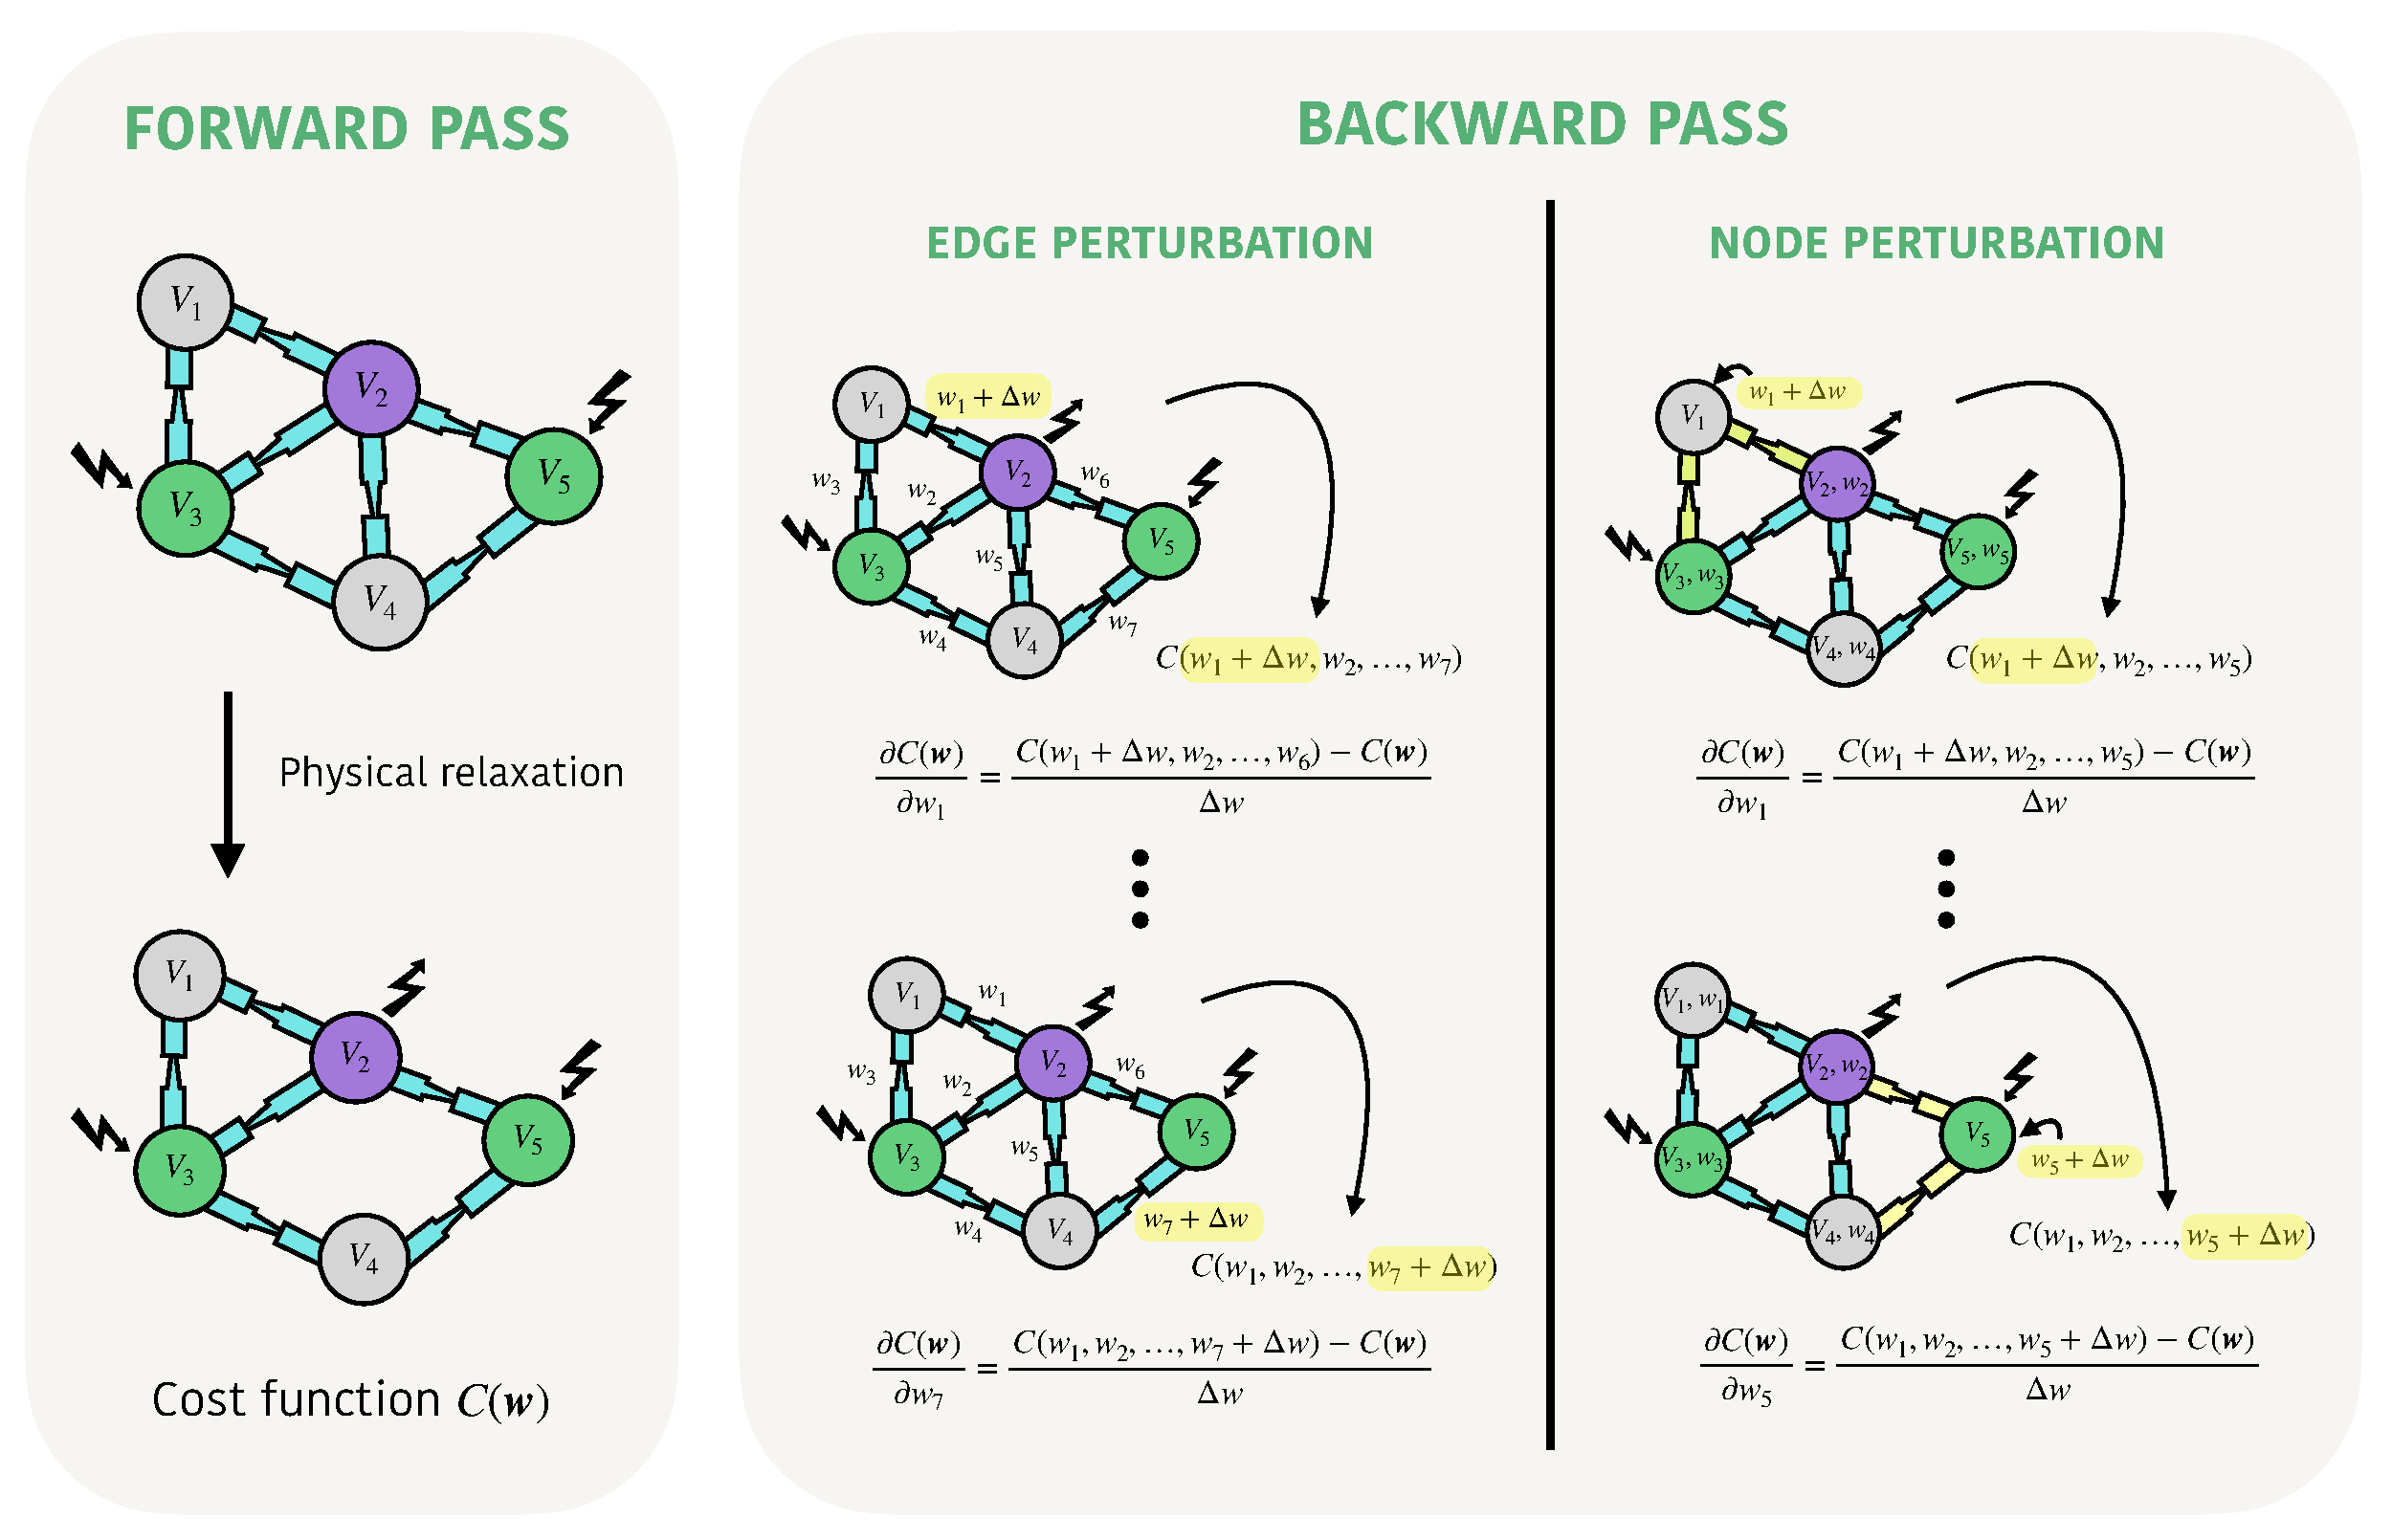
\includegraphics[width=\textwidth]{plots/training/training_scheme.pdf}
    \caption{Scheme representing the two phases of the training algorithm, they are iteratively performed for a selected number of training steps.}
    \label{fig:training_scheme}
\end{figure*}
We developed a training algorithm that makes use of the physical dependencies of memristor conductivity on both external stimuli and geometric properties to implement a physical neural network. These dependencies allow us to interpret such physical parameters as tuneable weights, analogous to standard artificial neural networks, and to encode learning directly into the physical structure of the system. As in traditional ANNs, the goal of the training algorithm is to modify these weights so that the network maps a given set of inputs to a corresponding set of desired outputs. In the case of the memristor network considered here, training aims to produce specific voltage values at designated output nodes, given fixed voltage inputs at the input nodes.

Crucially, the physical quantities that influence memristor conductance fall into two distinct categories: external stimuli, such as pressure or concentration, that are applied to the nodes, and geometric parameters, such as channel length or base radius, that are defined on the edges. As a result, we distinguish between two types of training strategies: \emph{node-defined weight training}, as illustrated in \cref{fig:two_types_weights}(a), and \emph{edge-defined weight training}, as shown in \cref{fig:two_types_weights}(b).

A modification to any of these weights affects the network's behaviour by altering the functional form of the memristor’s steady-state conductance, $g_{\infty}(\boldsymbol{\Delta})$, which depends on the local potential, pressure, and concentration drops across the device. Importantly, the functional shape of $g_{\infty}$ plays a role in determining the network’s dynamics and ultimate steady state, as illustrated in \cref{app:dyn_evol_steady_state}.

In this work, we focus on training a single property as the weight, while keeping all other parameters fixed as initially defined. For example, we may select an external stimulus, such as the imposed pressure or the density at each node. Alternatively, we can choose the length or base radius of the channel. The training process is carried out by iterating a scheme, illustrated in \cref{fig:training_scheme}, which consists of two phases: a forward pass and a backward pass.

\begin{figure*}[t]
    \centering
    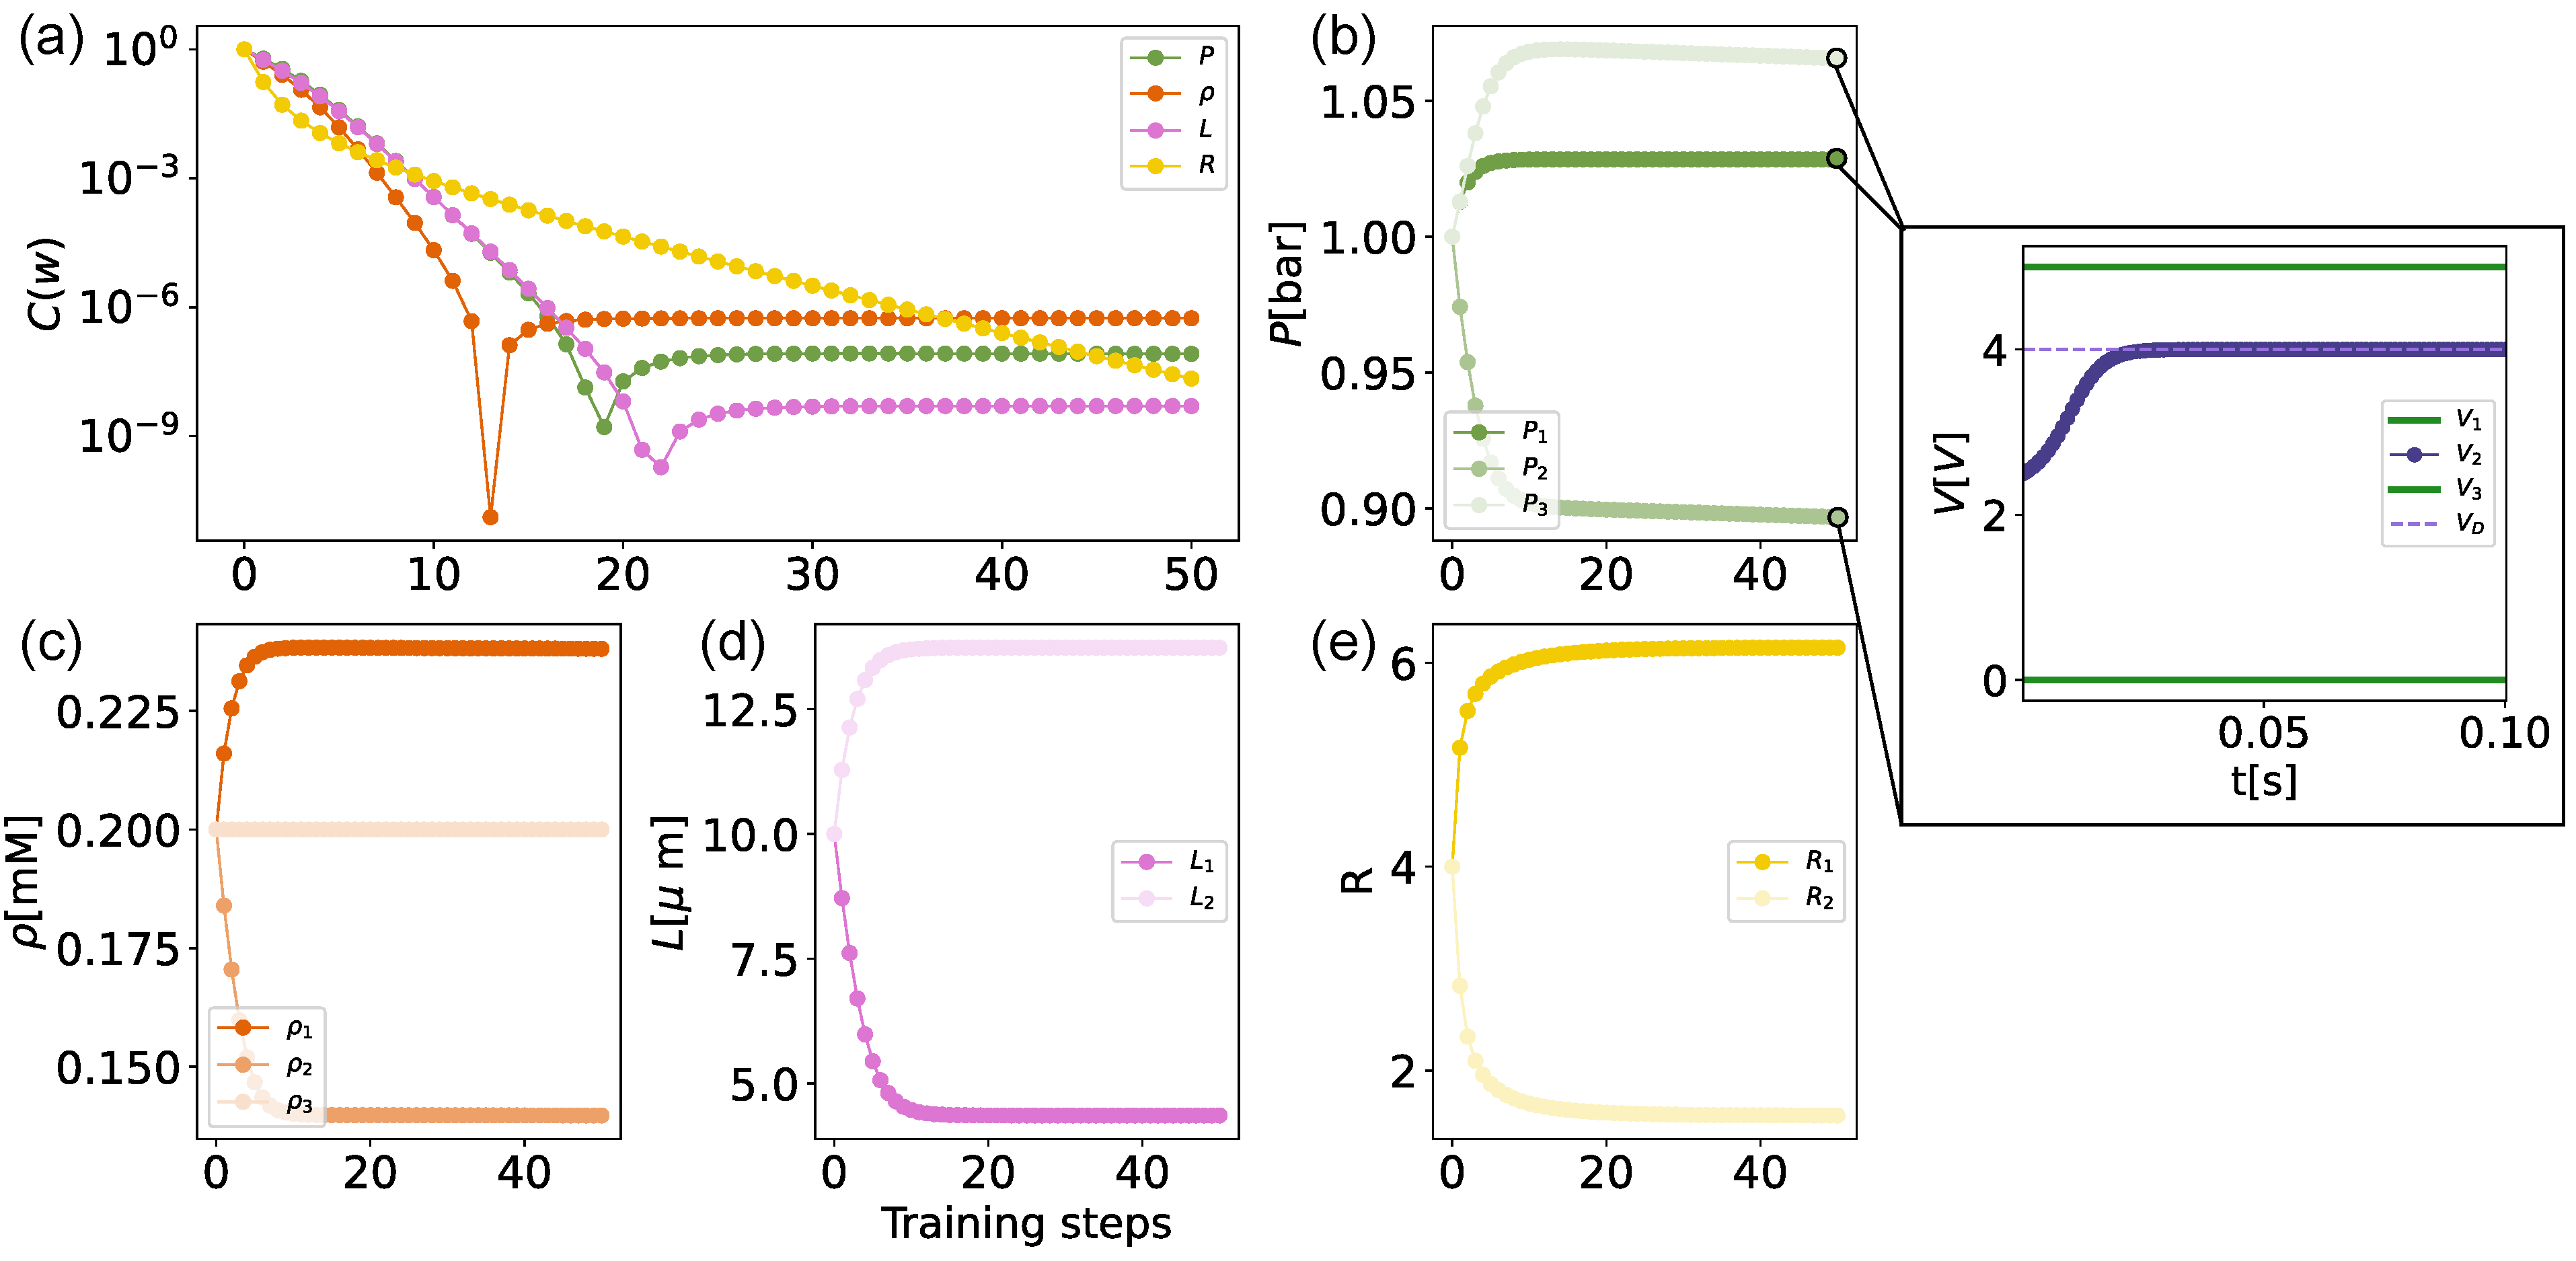
\includegraphics[width=1.7\columnwidth]{plots/voltage_divider/mse_weights_vd.pdf}
    \caption{(a) Behaviour of the cost function $C(\boldsymbol{w})$ during the training of the memristor voltage divider. Different colors indicate that the training is done with a specific choice of training weights, as indicated in the legend. Learning rates are set to $[3\cdot 10^{-6}, 3\cdot 10^{-6}, 5\cdot 10^{-4}, 100]$. (b) Pressures imposed on the three nodes of the voltage divider during training. The inset shows the relaxation to the steady state of the output voltage $V_2$ to the desired value $V_2^D$ when the pressures imposed are the values obtained in the last training step, and the input nodes are stimulated with fixed voltage. (c) Ion concentration densities imposed on the three nodes of the voltage divider during training. (d) Length of the memristors during training. (e) Base radius of the memristors during training.}\label{fig:mse_weights_vd}
\end{figure*} 
In the forward phase, the network is fed with specific electric potentials in the input nodes. Following both circuit laws and memristor's dynamics, the network reaches a steady state where electrical potentials can be measured in the output nodes. Clearly, the output of the network depends on the set of weights imposed on the network $\boldsymbol{w}$, regardless them being node or edge defined. The value of the outputs can be used to quantify the status of the network, meaning how much its answer differs from the desired one. Specifically, we define a \emph{cost function} that computes the difference squared between the voltage in the output nodes and the values of desired voltages
\[
C\left( \boldsymbol{w} \right) = \sum_{i \in \Lambda} \brac{V_i\brac{\boldsymbol{w}} - V_i^D}^2,
\label{eq:cost_func}
\]
where $\Lambda$ represents the set of indices belonging to the output nodes, $V_i\brac{\boldsymbol{w}}$ the voltage measured on the output nodes and $V^D$ is a vector containing the values of desired output nodes.

The backward phase has the fundamental purpose of finding a set of weights that minimize the cost function. We follow the method of the      \textit{steepest descent}, for which the update of the weights from one training step $s$ to the following $s+1$,
\begin{equation}
\boldsymbol{w}^{s+1} = \boldsymbol{w}^{s} - \alpha \boldsymbol{\nabla}C\brac{\boldsymbol{w}},
\label{eq:weight_update}
\end{equation}
results in a decrease in the cost function until a minimum is reached, for sufficiently small values of $\alpha$ \cite{steepest_descent_book}. The gradient in the update rule
\begin{equation}
    \boldsymbol{\nabla}C\brac{\boldsymbol{w}} = \left[ \frac{\partial C(\boldsymbol{w})}{\partial w_1}, \dots, \frac{C(\boldsymbol{w})}{\partial w_M}  \right],
    \label{eq:gradient_cost_func}
\end{equation}
is computed using a \textit{finite differences method} for each $m$ component
\begin{equation}
\frac{C(\boldsymbol{w})}{\partial w_m} = \frac{C\brac{w_1, \dots, w_m +\Delta w, \dots, w_M}-C\brac{\boldsymbol{w}}}{\Delta w},
\label{eq:gradient_cost_func_comp}
\end{equation}
where $\Delta w$ is a small increment, that we always set such that $w_m(t=0)/\Delta w = 10^{3}$.

In the training algorithm, we first initialize the system with the memristor parameters specified in \cref{sec:memristor_network}, an initial pressure of $1\text{bar}$ and concentration of $0.2\text{mM}$ at each node. With the knowledge of input and desired output voltage values, it is possible to perform the first forward pass, from which we obtain the cost function $C\brac{\boldsymbol{w}}$, that we store since it is needed in the computation its gradient. Subsequently, we proceed with the backward pass. We compute each entry of the gradient in \cref{eq:gradient_cost_func} by selecting the corresponding weight, a node or an edge parameter, increment its value of $\Delta w$ and applying a forward step to obtain the corresponding entry of $C\brac{w_1, \dots, w_m +\Delta w, \dots, w_M}$. With the stored value of $C\brac{\boldsymbol{w}}$, we are able to compute the component of the gradient as in \cref{eq:gradient_cost_func_comp}, and use the gradient to calculate the weight update in \cref{eq:weight_update}. 

Although performed numerically in this work, we highlight that the feedforward pass is a physical process in which the system naturally relaxes to its steady state. Moreover, also the backward pass we use can be translated to a physical event since involves performing the forward pass a number of time as the number of the weights. Once the gradient of the cost function is determined and stored, only the simple algebraic calculations of \cref{eq:weight_update} are left to be computed. We propose this method as a hybrid physical and in-silico training algorithm, as a future experimental approach to the problem.


\subsection{\label{sec:train_memr_vd}Training a Memristor Voltage Divider}
A voltage divider is an electrical circuit made of three nodes connected in series by two resistances, that returns a fraction of the input voltage. Given the simplicity of its structure, we use it as an initial playground for the training algorithm described above. Specifically, we replace the resistances with memristor channels, to be trained such that giving $V_1 = 5V$ and $V_3 = 0V$ as inputs, we get $V_2^D = 4V$ as output. In \cref{fig:vd_scheme} a schematic of the memristor voltage divider is shown.
\begin{figure}[t]
    \centering
    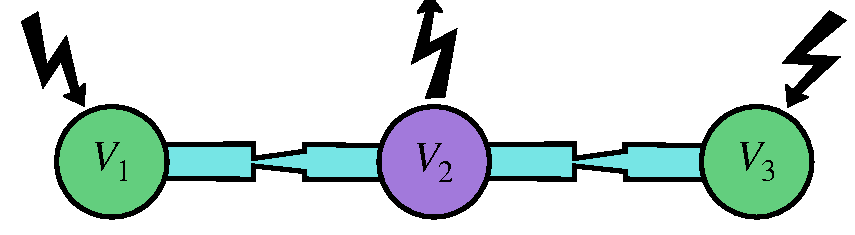
\includegraphics[width=0.5\columnwidth]{plots/voltage_divider/vd_scheme.pdf}
    \caption{Schematical representation of a memristor voltage divider.}\label{fig:vd_scheme}
\end{figure} 

We initialize the system with pressures $P_1 =  P_2 = 1 \text{bar}$ and ion concentration $\rho_1 = \rho_2 = 0.2 \text{mM}$ on each node, length $L_1 = L_2 = 10\mu \text{m}$ and base radius  $R_{b1} = R_{b2} = 200 \text{nm}$ on each edge. After choosing one of these four physical quantities as training parameter $\boldsymbol{w} = \brac{w_1, w_2}$, we implement the training as described in \cref{sec:training} that modifies them, while the other parameters are kept constant. 
\begin{figure}[b]
    \centering
    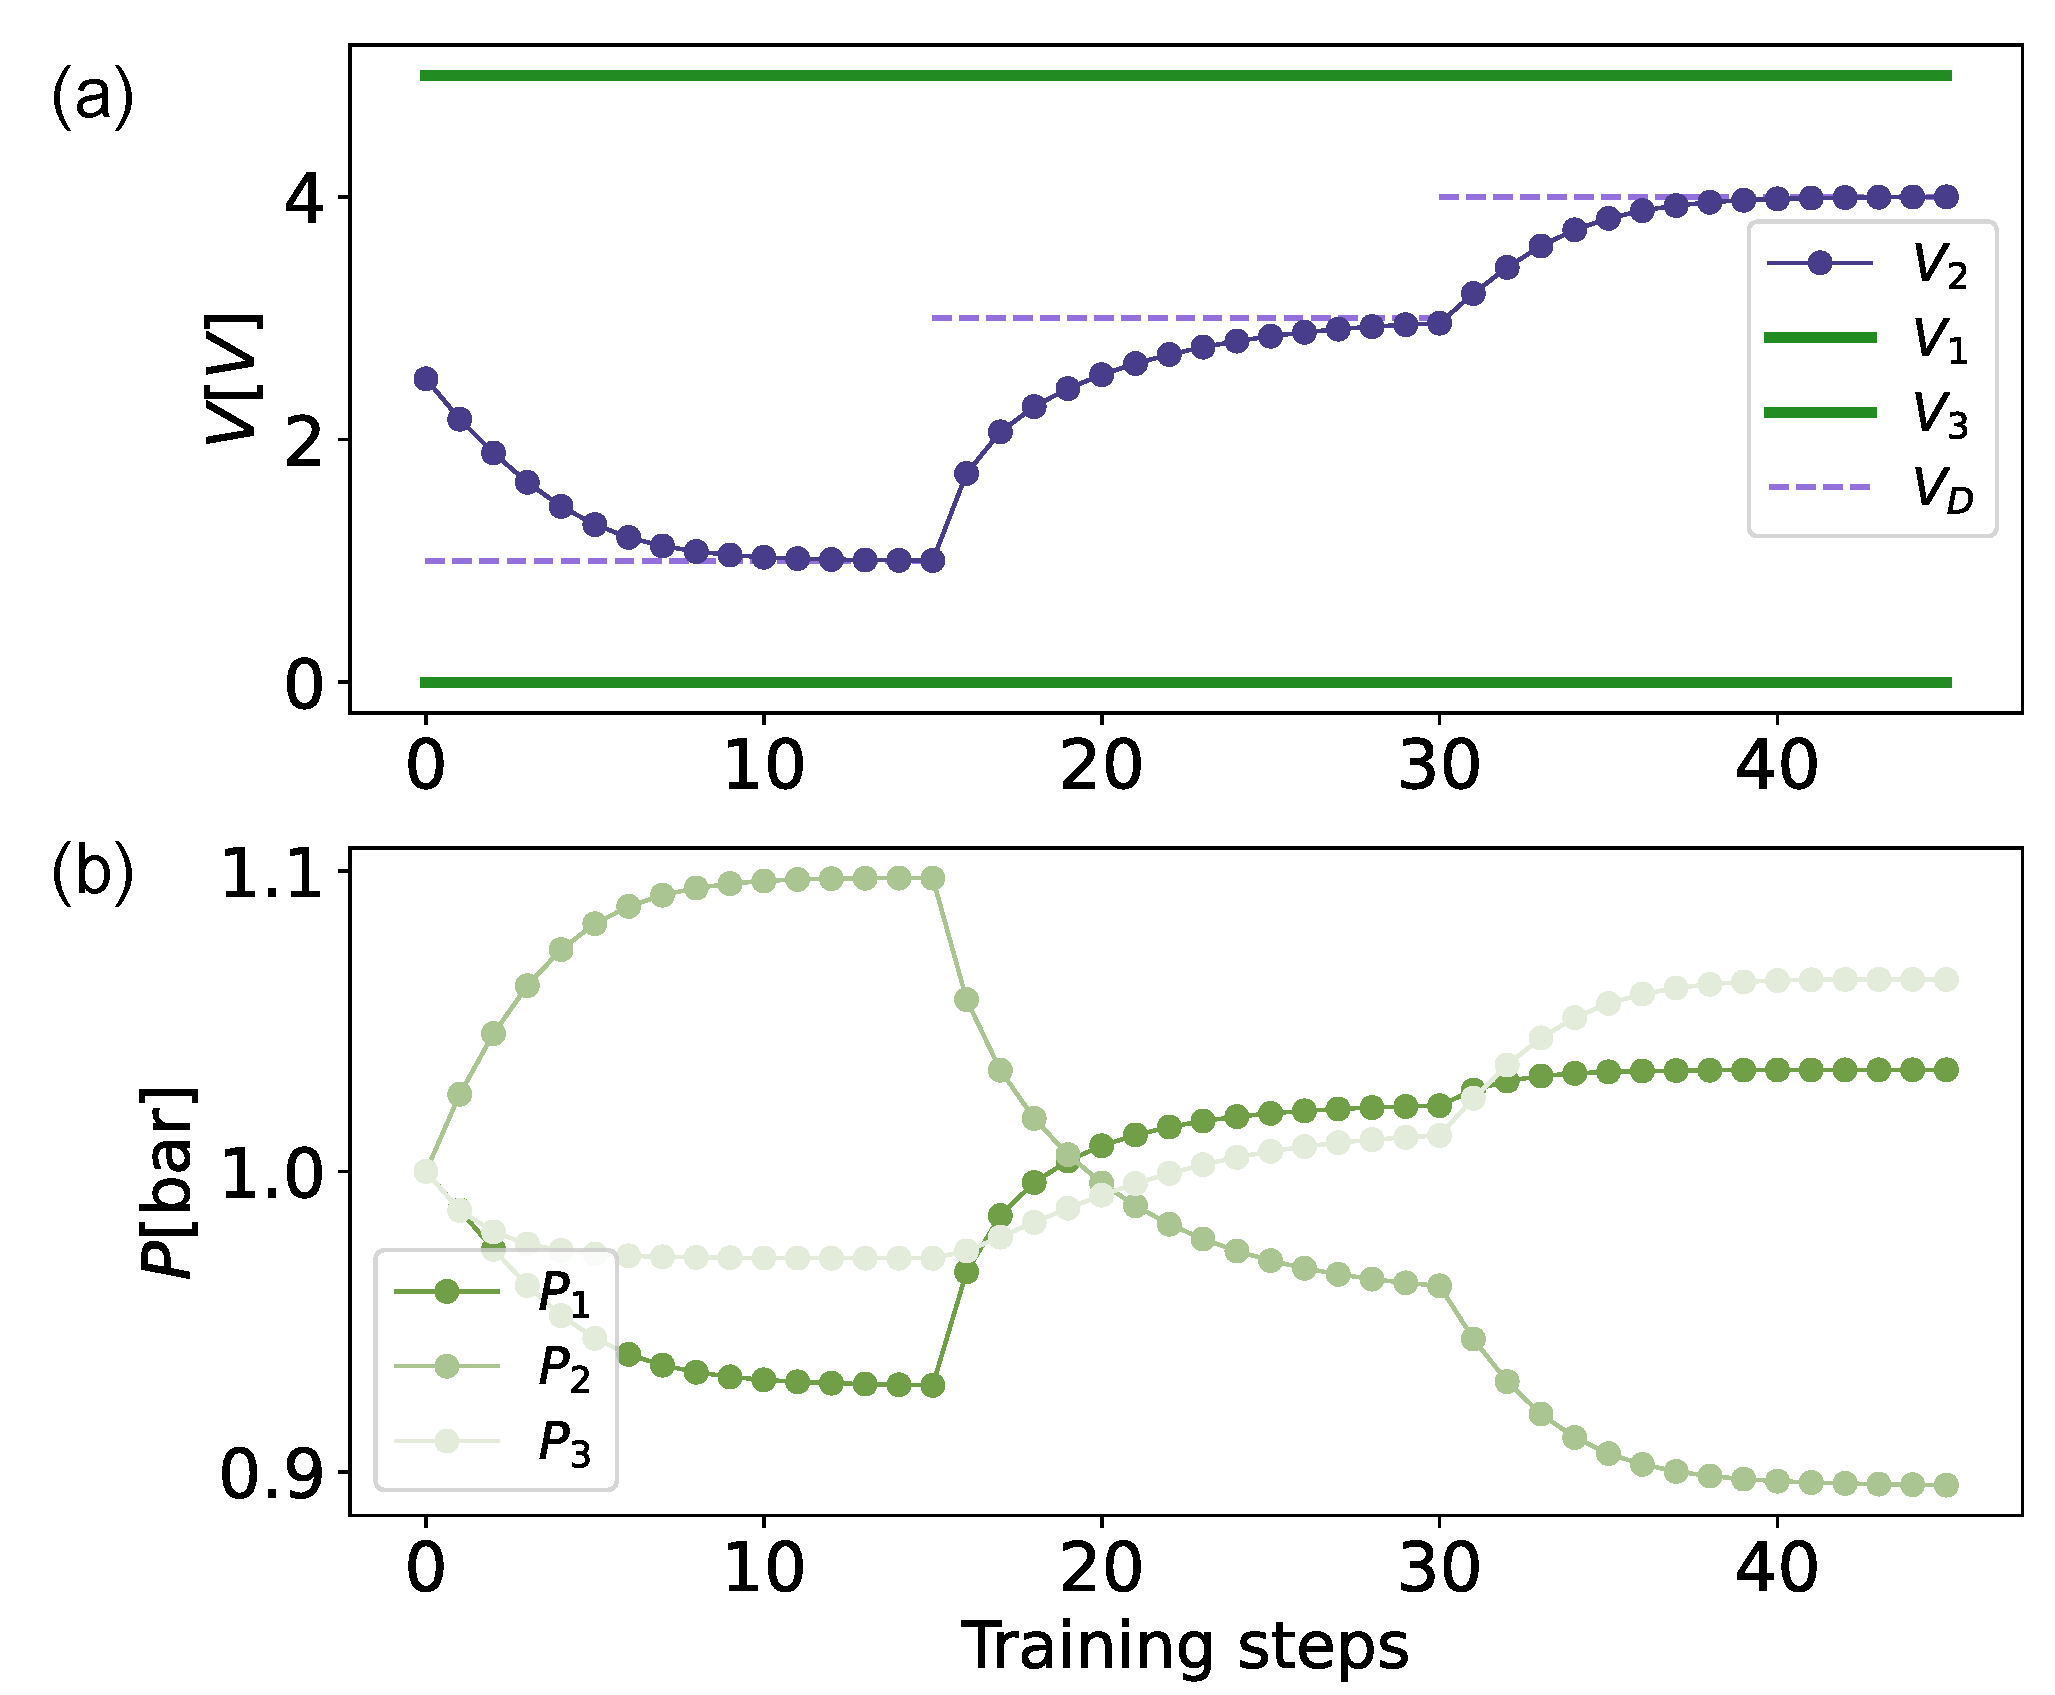
\includegraphics[width=0.8\columnwidth]{plots/voltage_divider/evolution_targets.pdf}
    \caption{(a) The training of a memristor voltage divider to a set of desired voltage outputs, indicated by dashed light purple lines. The output voltage $V_2$, indicated by dark purple dots, adapts to the desired output during the training. The input voltages $V_1$ and $V_3$ are constant at $5V$ and $0V$ respectively. (b) The dots with different shades of grey show the values of pressures, chosen as weights, imposed on the three nodes during training.}\label{fig:evolution_targets}
\end{figure}
In \cref{fig:mse_weights_vd}(a) we show that the cost function normalized to its initial value decreases of many order of magnitude during the training for each of the chosen weight. The values of the chosen set of weights simultaneously changes from the initial condition, as shown in \cref{fig:mse_weights_vd}(b)-(e), adjusting the behaviour of the network to the desired one. If the values of a chosen type of weight at the end of the training are imposed to the network together with the voltage inputs, the network will autonomously relax to a steady state that coincides with the desired state. To exemplify this point, the inset in \cref{fig:mse_weights_vd}(b) shows the physical relaxation of the voltage divider when the trained values of pressure, which correspond to the three values in the last training step, are imposed on the nodes together with the constant inputs voltages. The inset shows that the output voltage $V_2$ autonomously relaxes to the desired value of $V_2^D=4V$ in a time scale characteristic of the memristor.

In order to investigate the adaptability of the algorithm, we trained the system with a set of three consequent desired voltages $V_2^D=\{1V, 3V, 4V\}$. In \cref{fig:evolution_targets} we show how the output voltage $V_2$ subsequently adapts to the desired voltages during the training of the pressures in the nodes, the evolution of which can be seen in \cref{fig:evolution_targets}(b). It is evident that the system can be retrained at any stage to a new desired objective making it reusable. Any other weight type can be chosen, depending on the necessity.  


\subsection{\label{sec:train_memr_nw}Training a memristor network}

To generalize the training objective, we consider a memristor network constructed with a more complex geometry. \cref{fig:mse_general}(a) illustrates a network with three input nodes and two output nodes. The network is trained to produce output voltages of $[3,V, 4,V]$ when provided with input voltages of $[0,V, 2,V, 5,V]$.  Reaching a desired input-output voltage mapping in a generic electric circuit can be useful for various electronic purposes \cite{voltage_controlled_oscillator, onchip_powerdistributed}. 

\begin{figure}[h]
    \centering
    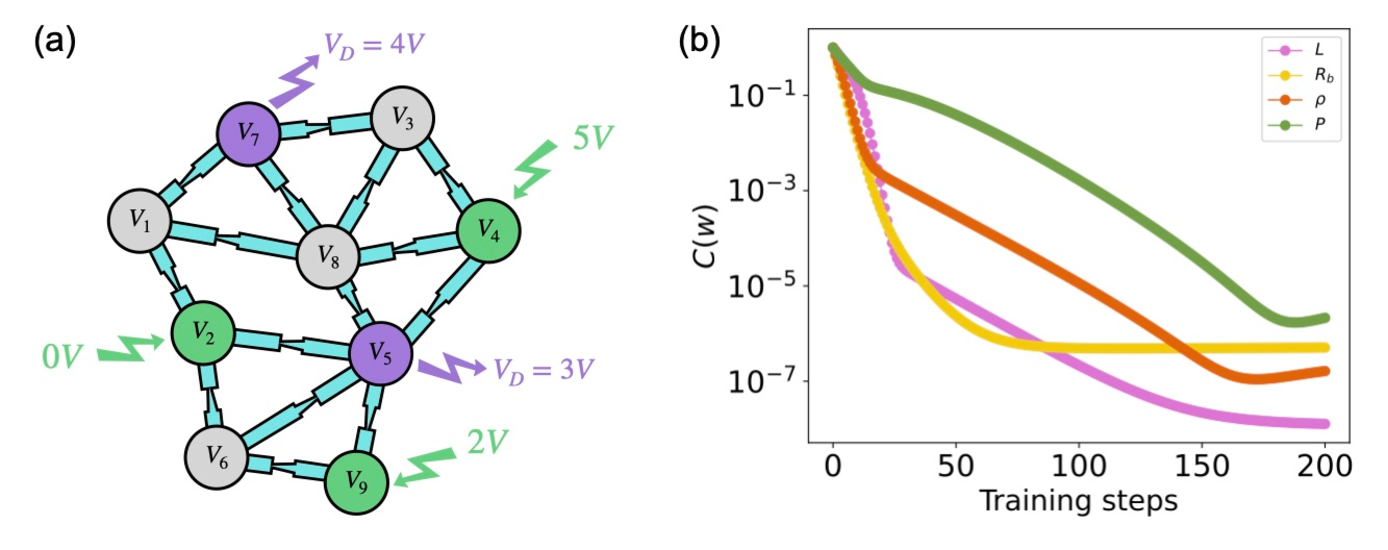
\includegraphics[width=0.5\textwidth]{plots/general_network/mse_general.pdf}
    \caption{(a) Generic network with $9$ nodes and $15$ edges with inputs $[V_{2}, V_{4}, V_{9}] = [0V, 2V, 5V]$ and desired outputs $[V_{5}^D, V_{7}^D] = [3V, 4V]$, learning rates $[10^{-3}, 1, 10^{-4}, 10^{-3}]$. (b) Cost function during training of generic graph for input-output mapping task. The different colors indicate different weight choice.}\label{fig:mse_general}
\end{figure} 

The result of the training is presented in \cref{fig:mse_general}(b), which shows how the cost function responds to the weight updates performed in the algorithm, for each of the four different weights. All of the possible different choices of weight result in a trained set that decreases the initial error of many orders of magnitudes. 

\subsection{\label{sec:linear_regression}Linear Regression}
\begin{figure*}[t]
    \centering
    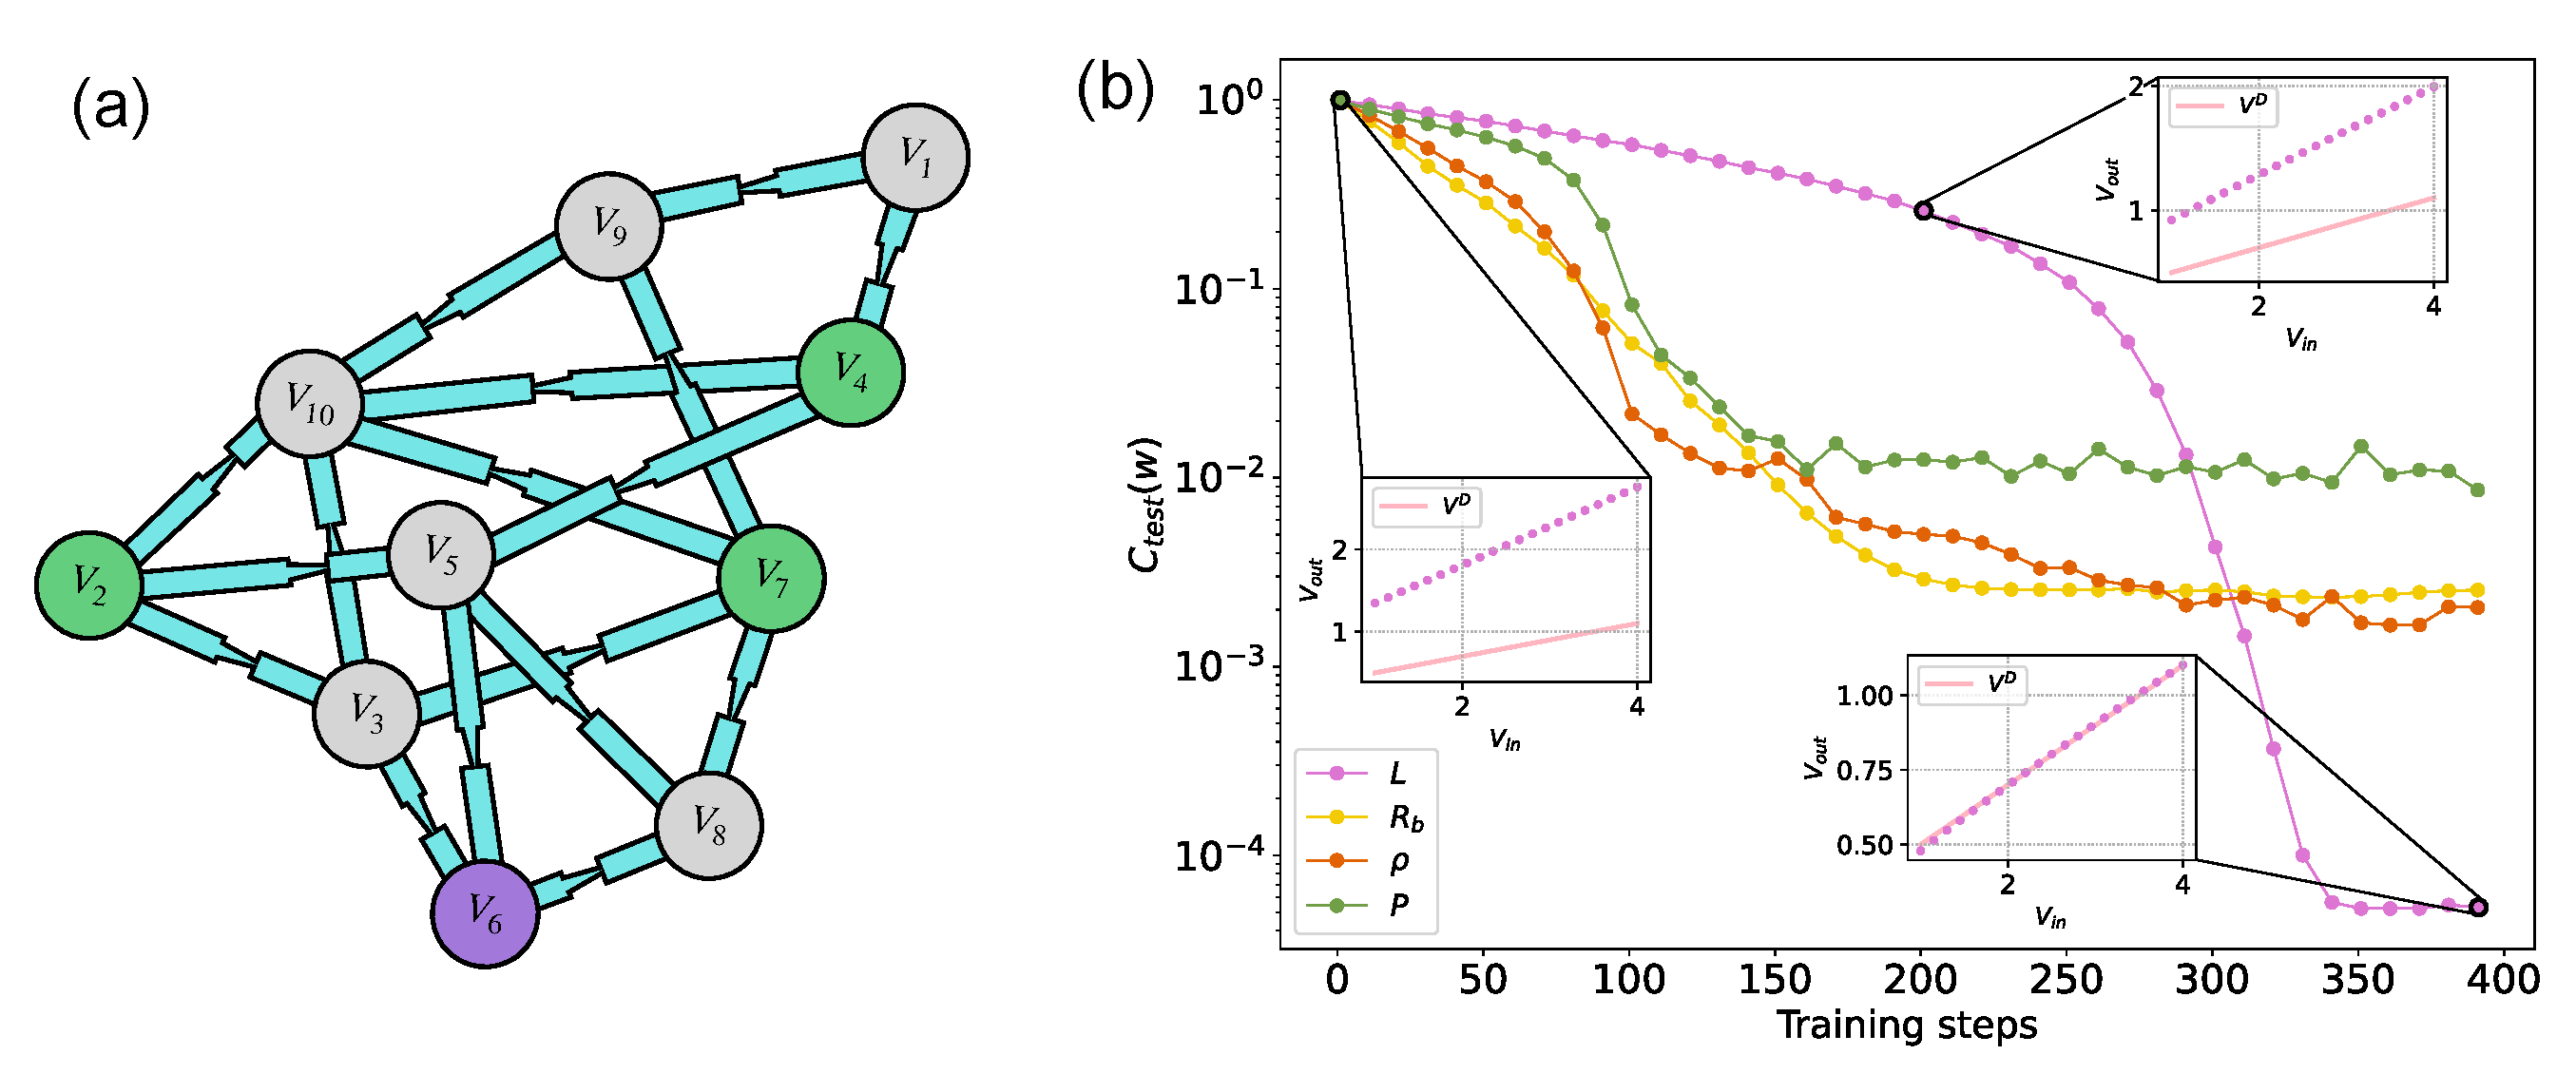
\includegraphics[width=0.85\textwidth]{plots/regression/regression_G00010001.pdf}
    \caption{(a) Network geometry used for linear regression training. The network comprises $17$ edges connecting $10$ nodes, including one output node (purple dot) and three input nodes (green dots). Among the three input nodes, one is used to ground the circuit ($V_2 = 0V$), one ($V_4$) provides a constant voltage source for bias, and the remaining one ($V_4$) is used to input the training data point. For the four weight types (channle length, base radius, ion density and pressure), we used as constant voltage input $V_4 = [11V,4V,4V,11V]$ and learning rates $[2\cdot 10^{-7}, 1\cdot 10^{-6}, 1\cdot 10^{-4}, 2\cdot 10^{2}]$. (b) Test cost function evaluated every $10$ training steps for four different weight choices. Insets show visual representations of the network’s output trained with varying channel lengths at three different training steps.}\label{fig:lin_regr1}
\end{figure*}

We broaden the training capability of the network by including a linear regression task, where, in its simplest form, the network is trained to give potential output $V_{\text{out}}$ in a certain node of the network, related to the input potential $V_{\text{in}}$ via a linear relationship
\begin{equation}
    V_{\text{out}} = \text{a} V_{\text{in}} + \text{b}.
\label{eq:linear_relationship}
\end{equation}
We generate two sets of data, a training set $ \{ V_{\text{in}}^{(j)}, V_{\text{out}}^{(j)} \}_{j=1}^{N_{\text{train}}}$ and a test set $ \{ V_{\text{in}}^{(j)}, V_{\text{out}}^{(j)} \}_{j=1}^{N_{\text{test}}}$, where $N_{\text{train}}$ and $N_{\text{train}}$ denote the number of training and test samples, respectively. To create the training set, a sequence of input voltages is randomly sampled from the interval $[1V, 4V]$, and the corresponding output voltages are computed using equation \cref{eq:linear_relationship}, ensuring that the input-output pairs satisfy the desired relationship.
The test set is constructed in a similar way, but uses $N_{\text{test}}=20$ input values that are evenly spaced within the same interval. Their corresponding outputs are also computed using equation \cref{eq:linear_relationship}. Note that the training and test sets contain different input values.

The training algorithm described in \cref{sec:training} can be slightly adapted to support this training objective. At each training step, an input-output voltage pair, or sets, is selected from the training set and used as the input voltage and target output in the algorithm. This differs from the original algorithm, where the same input-output pair was presented at every step.

Therefore, at each training step $ j \in[1, N_{\text{train}}] $, the cost function used to compute the gradient in \cref{eq:gradient_cost_func} is adapted to
\[
C_j(\boldsymbol{w}) = \left[ V_{\text{out}}(\boldsymbol{w}) - V_{\text{out}}^{(j)} \right]^2,
\]
where $ V_{\text{out}}(\boldsymbol{w}) $ is the measured output voltage for the selected input, and $ V_{\text{out}}^{(j)} $ is the corresponding target output in the training set. This expression corresponds to a simplified version of \cref{eq:cost_func} for the case of a single output node.

\begin{figure*}[t]
    \centering
    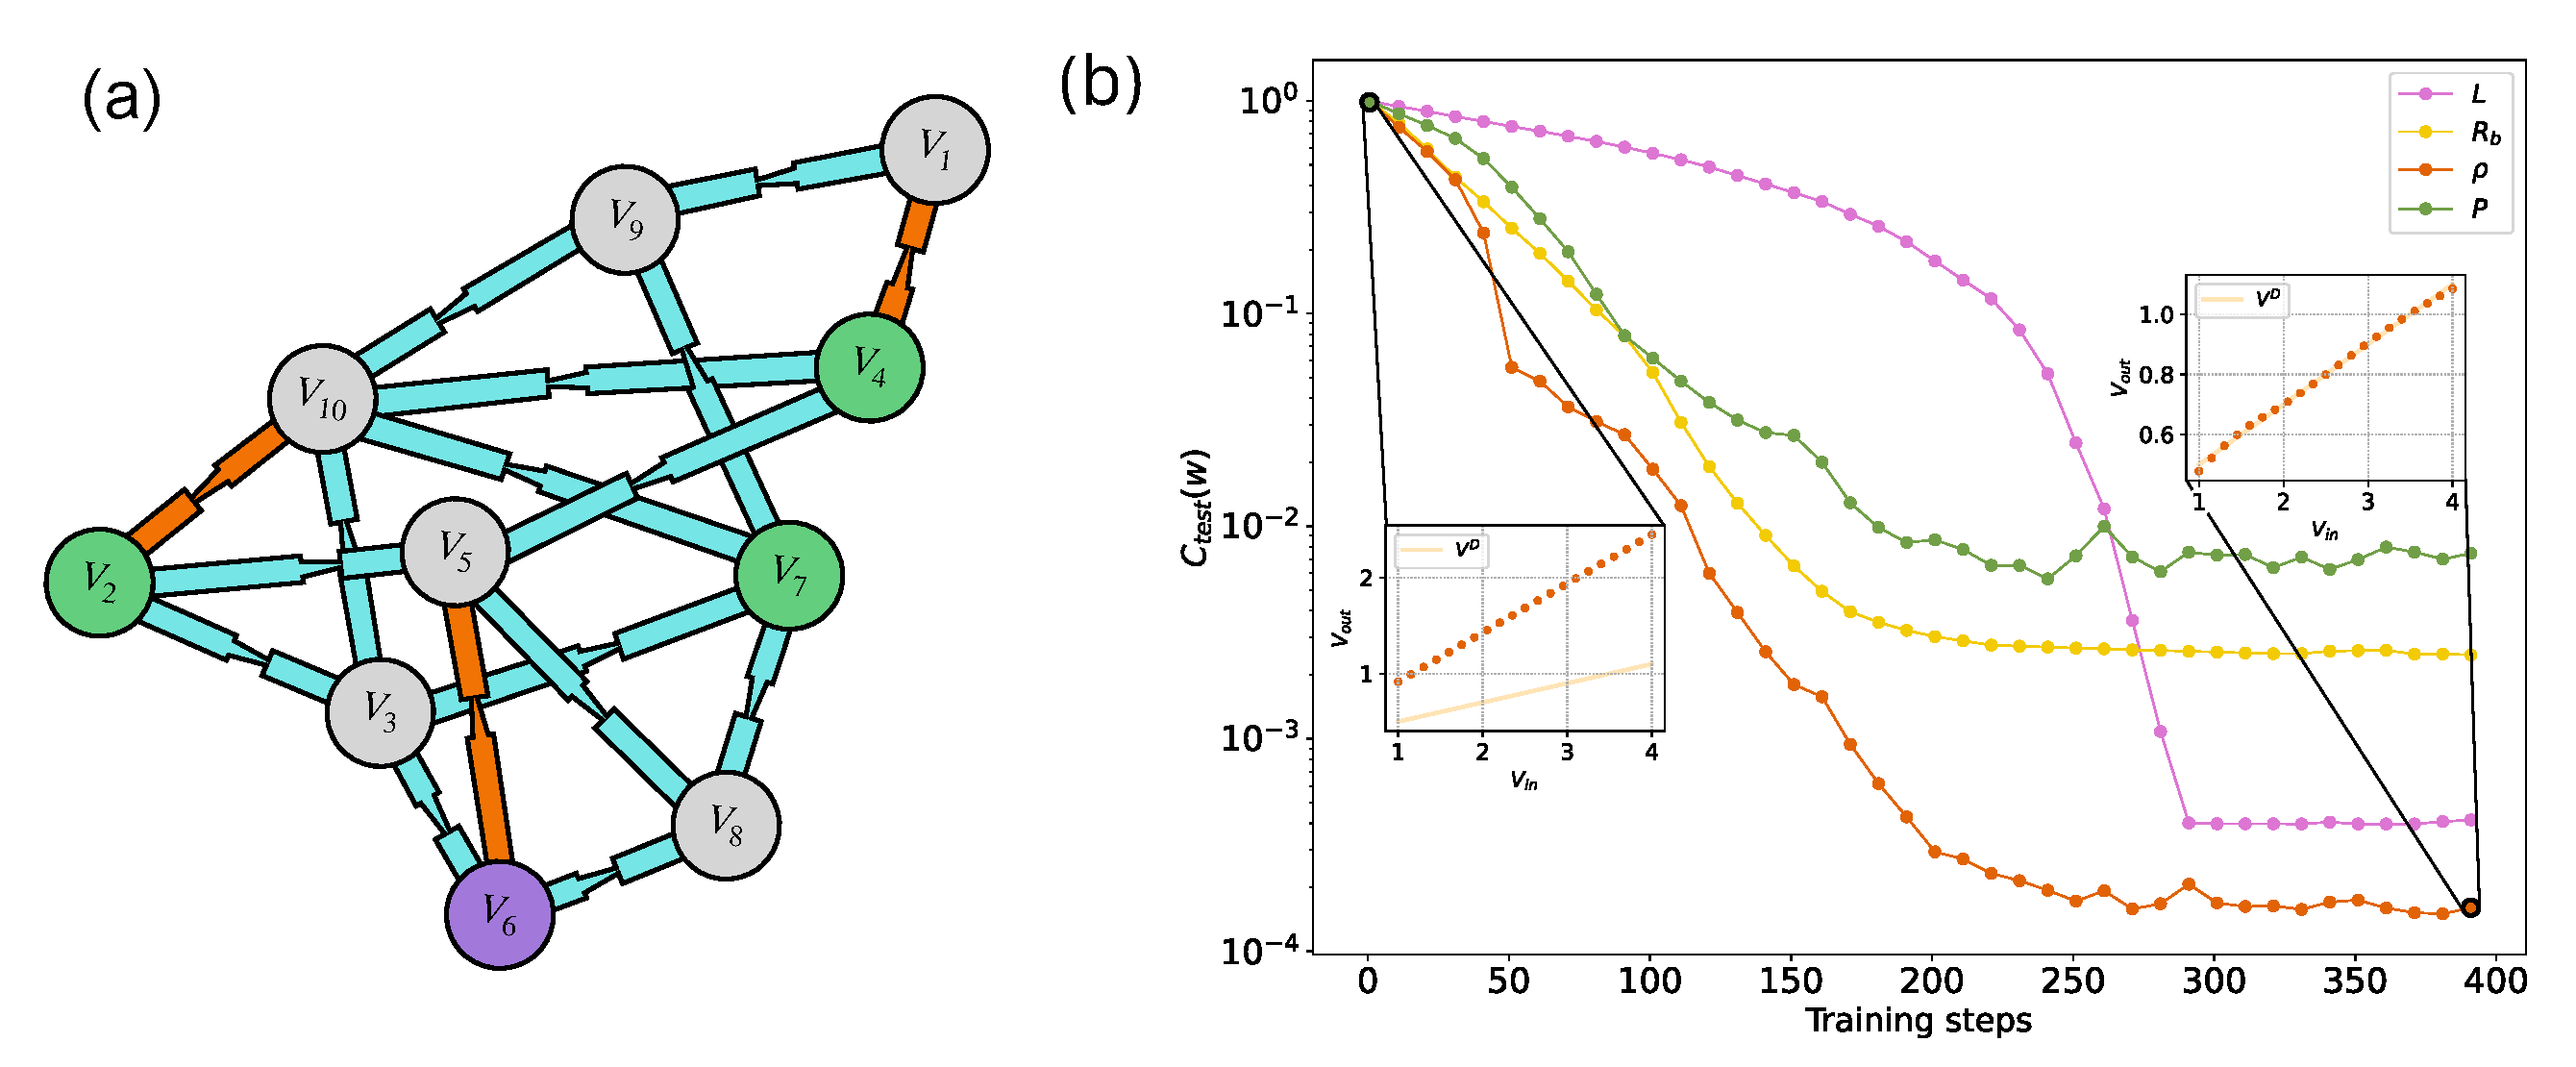
\includegraphics[width=0.85\textwidth]{plots/regression/regression_G00010002.pdf}
    \caption{(a) Network geometry used for linear regression training. It is equivalent to the geometry shown in \cref{fig:lin_regr1}, but the direction of the memristors highlighted in orange has been inverted. For the four weight types (channle length, base radius, ion density and pressure), we used as constant voltage input $V_4 = [11V,4V,4V,11V]$ and learning rates $[3\cdot 10^{-7}, 1\cdot 10^{-6}, 9\cdot 10^{-4}, 2\cdot 10^{2}]$. (b) Test cost function evaluated every $10$ training steps for four different weight choices. Insets show visual representations of the network’s output trained with varying node ion density at two different training steps.}\label{fig:lin_regr2}
\end{figure*} 
To evaluate how well the algorithm performs during training, we compute the \emph{test cost function} $ C_{\text{test}} $ over the entire test set. If $ \boldsymbol{w} $ denotes the weight vector at a given training step, the test cost is defined as
\[
C_{\text{test}}\left( \boldsymbol{w} \right) = \sum_{j=1}^{N_{\text{test}}} \left[ V_{\text{out}}(\boldsymbol{w}) - V_{\text{out}}^{(j)} \right]^2,
\]
which sums the squared differences between the measured and target output voltages at each test point. For each input $V_{\text{in}}^{(j)}$ in the test set, the voltage $ V_{\text{out}}(\boldsymbol{w}) $ is the output produced by the network with weights $ \boldsymbol{w} $, while $ V_{\text{out}}^{(j)} $ is the desired output. This test cost is used for performance evaluation and is not involved in the training process.

Since the task is more demanding than a single input-output mapping, we use a larger network with more degrees of freedom. \cref{fig:lin_regr1}(a) shows the graph selected for the regression task. It consists of 20 edges and 10 nodes, three of which are inputs and one is an output. Among the three input nodes, one is set to ground and another to a constant value, in order to enable the training of a linear function with an offset. For the training objective, we aim to train the network to fit the line $V_{\text{out}} = 0.2 V_{\text{in}} + 0.3$ over the input voltage range $[1V, 5V]$.

The performance of the algorithm on this task is shown in \cref{fig:lin_regr2}(b), where the learning rates for the different weights have been fine-tuned to prevent overshooting while still maintaining comparable convergence speed. From the behaviour of the cost function, it is evident that the choice of weight type has a decisive impact on the network’s ability to learn a complex task. Specifically, training the lengths of the channels on the edges results in successful convergence, whereas training the node pressures proves to be less efficient. For a visual interpretation, insets in \cref{fig:lin_regr1}(b) show the state of the training at three different time steps when the selected weight is the length of the channel.

To study the influence of memristor orientation on training performance, we retained the same network geometry but inverted the orientation of some memristors, as shown in \cref{fig:lin_regr2}(a). Specifically, if in the original configuration the base of a memristor pointed to one node and the tip to another, we reversed this direction. This modification significantly affects the behaviour of the network. As shown in \cref{fig:lin_regr2}(b), the new orientation alters the trainability of different weight types: in this configuration, training node concentration leads to better performance, while training edge length becomes less efficient. The underlying reason is that inverting the orientation of a channel also inverts the sign of the external stimulus applied to it, since the stimuli are defined node-wise and the difference is always taken as ''base minus tip".

This reversal changes both the shape and the conductivity range over which the function $g_{\infty}(\boldsymbol{\Delta})$ is defined, thereby limiting or enabling the conductivity values the channel can reach. A network with well-oriented channels can therefore access conductivity ranges that make the training solvable, while a poorly oriented network may be constrained to regions where solutions are not found. To exemplify this point, Figure 2 of Ref.\cite{Rene_PressureSensitive} shows $g_{\infty}$ as a function of pressure for positive and negative potential drops, assuming a zero concentration drop. The plot reveals two completely disjoint conductivity ranges depending on the sign of the potential drop, which explains why training on pressure alone may be challenging. This highlights the need for deeper exploration of network geometry when selecting the type of weight to train. In this regard, we observe that the edges whose orientation was inverted are directly connected to either the input or the output nodes. This suggests that particular attention should be given to these edges in future explorations, as they may have a bigger impact on trainability.

\section{\label{sec:concl}Conclusions}

We proposed a physical neural network composed of nodes connected by aqueous memristors. These devices exhibit conductance that responds to external stimuli of various physical natures, such as electrical, mechanical, and chemical. Additionally, their conductivity is sensitive to changes in the geometric parameters of their channel-like structure. Our motivation for using these devices lies in the ability to exploit these dependencies to control the conductance of each memristor in the network. This enables us to manipulate an input electrical signal in a programmable way, according to a specific computational objective.

To this end, we developed a training algorithm that targets one of the physical parameters influencing conductivity and treats it as the analog of a weight in a standard machine learning framework. The electrical signal is used as both input and output, while other types of signals or geometric dependencies are used to adjust the network during training.

The training process consists of two phases. The first is an inference phase, in which input voltages are applied to the system and the circuit is allowed to physically relax to a steady state. At this point, the output voltages can be read. Ideally, these outputs should match a predefined set of target values reflecting the training goal. In the second phase, the update phase, the weights are adjusted to minimize a cost function based on the difference between the actual and desired outputs. By iteratively applying this procedure, the network is gradually tuned to achieve the desired input-output behaviour.

The inference phase is entirely physical, as the system evolves naturally to its steady-state response when inputs are applied. In contrast, the update phase is only partially physical. The weight update relies on estimating the gradient of the cost function using a finite-differences method, following a steepest descent rule. Specifically, each weight is perturbed slightly, and the resulting change in the cost function is computed. The gradient is then approximated by taking the difference in cost between the perturbed and unperturbed configurations, divided by the magnitude of the perturbation. While an external computer is required to store and coordinate the gradients for each weight, the values themselves can be obtained through physical measurements of the system's output under the two conditions. This structure allows for a mostly physical implementation of learning, with digital support.

As a first simple application, we tested the algorithm on a voltage divider, training the network to produce a specific fraction of the input voltage at the output node. The training was successful across all four selected weight types: pressure drop, concentration gradient across the memristor, length of the memristor, and its base radius.After selecting a particular weight type, we further demonstrated that the network, once trained to achieve a specific objective, could be retrained to a different target with similar training speed. This result indicates that the algorithm is both adaptive to new training objectives and largely independent of the initial weight configuration.

Training larger and more complex memristor networks is also feasible with the algorithm we proposed. We demonstrated that a network composed of 9 nodes and 15 edges can be successfully trained for more elaborated input-output voltage mapping using all the weight types considered.

We then challenged a more complex network, with 10 nodes and 17 edges, to perform a linear regression task with an offset. In this setting, we observed that the trainability of the network using a specific weight type strongly depends on the network's geometry. First, we showed that different geometries yield different final training accuracies when using the same weight type. Then, keeping the geometry fixed, we demonstrated that the orientation of the memristors also plays a crucial role: reversing the direction of just three memristors connected to either input or output nodes improved the training precision when using concentration as the trained weight by three orders of magnitude.

Given that the expressiveness of deep neural networks grows exponentially with depth\cite{big_neuralnet1, big_neuralnet2}, we interpret the limitations encountered in training linear regression tasks as a consequence of the small size of the network. Larger networks offer more degrees of freedom and can, in principle, enable broader exploration of the solution space. However, their experimental realization becomes complex. In this work, we showed that an appropriately chosen geometry adapted to a specific training objective can be sufficient to make even a small networks trainable. A deeper analysis of the role of geometry in determining trainability is still needed in the context of physical learning. 

The core intention behind the algorithm is to enable a physically realizable neural network that requires minimal computational resources to operate. Thanks to the multiple physical dependencies of memristors, such as electrical, chemical, mechanical and geometrical factors, the algorithm supports a wide range of possible weight types. This flexibility makes it highly adaptable to various experimental scenarios, depending on which parameters are most accessible or controllable in a given setup. [.. examples of realizable system, cite literature].

\cleardoublepage
\appendix

\section{Dynamical evolution to the steady state \label{app:dyn_evol_steady_state}}

In this section, we provide a more detailed explanation of how a memristor network relaxes to its steady state. Alongside outlining the algorithm used to solve the circuit, we highlight the importance of the dependence on the functional form of the steady-state conductance, which itself is determined by the values of the weights. Selecting appropriate weights shapes the staedy state conductance function in such a way that the network naturally relaxes to a steady state aligned with the training objective.

For simplicity, we consider the voltage divider shown in \cref{fig:app_vd}, where the memristors are labeled as $ \m_1 $, connecting node 2 to node 1, and $ \m_2 $, connecting node 3 to node 2. We also denote the corresponding potential drops across each memristor as $ \Delta V_1 = V_2 - V_1$ and $ \Delta V_2  = V_3 - V_2$, respectively. To simplify, we set both the pressure difference ($ \Delta P $) and concentration difference ($ \Delta \rho $) to zero. In this example, we choose the channel length as the training weight.

\begin{figure}[H]
    \centering
    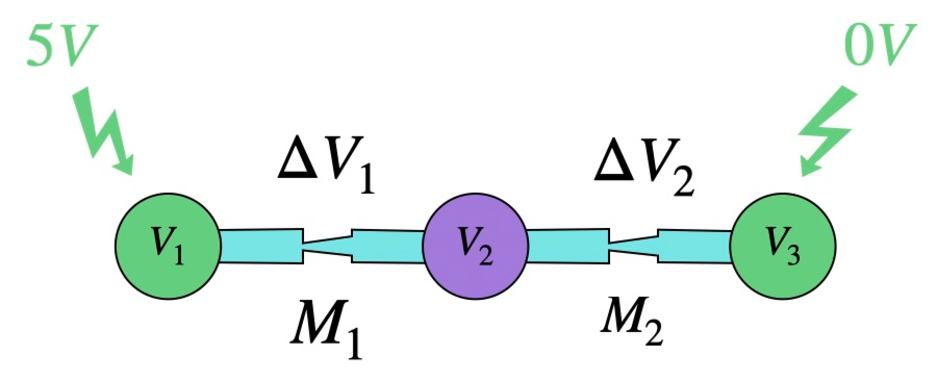
\includegraphics[width=0.5\columnwidth]{plots/appendixA/app_vd.pdf}
    \caption{Schematical representation of a memristor voltage divider. Two memristors, \( M_1 \) and \( M_2 \), connect two input nodes (green dots) with fixed voltages of \( 0\,\mathrm{V} \) and \( 5\,\mathrm{V} \), respectively, to a single output node (purple dot). Each memristor is subject to one external stimulus: the electric potential difference between the nodes it connects.
    }
    \label{fig:app_vd}
\end{figure} 
The dynamical evolution of the conductance of each memristor, discretized in time-steps of size $\Delta t$, reduces to the update rule:
\begin{equation}
g_{\m}(t + \Delta t) = g_{\m}(t) +
\frac{g_{\m,\infty}(\Delta V_{\m}(t)) - g_{\m}(t)}{\tau} \Delta t,
\label{eq:conduct}
\end{equation}
with initial condition $g_{\m}(t = 0) = g_0$. The potential drops across the memristors, $\Delta V_1(t)$ and $\Delta V_2(t)$, are computed from Kirchhoff's laws. In the case of a simple voltage divider ,see \cref{fig:app_vd}, these simplify to:
\begin{equation}
\Delta V_1(t) = \frac{5 g_2(t)}{g_1(t)+g_2(t)}, \qquad
\Delta V_2(t) = \frac{5 g_1(t)}{g_1(t)+g_2(t)},
\label{eq:potentials}
\end{equation}
Starting from initial values, the potential drops across the memristors are computed using Kirchhoff’s laws. These potential differences then drive the time evolution of the memristors’ conductances, following the discretized dynamical equation. The process—computing potential drops and updating conductances—is repeated iteratively until the conductance values converge to their steady-state counterparts. This iterative relaxation procedure is outlined in Algorithm 1.

\begin{algorithm}
    \caption{}
    \label{alg:relaxation}
    \begin{algorithmic}[1]
    \State \textbf{Input:} Initial conductance $g_0$, time step $\Delta t$, convergence threshold $\epsilon$, relaxation time $\tau$
    \State Initialize $g_1 \gets g_0$, $g_2 \gets g_0$, $t \gets 0$
    \While{not converged}
        \State Compute $\Delta V_1 \gets \frac{5 \cdot g_2}{g_1 + g_2}$
        \State Compute $\Delta V_2 \gets \frac{5 \cdot g_1}{g_1 + g_2}$
        \State $g_1 \gets g_1 + \frac{g_{\infty}(\Delta V_1) - g_1}{\tau} \cdot \Delta t$
        \State $g_2 \gets g_2 + \frac{g_{\infty}(\Delta V_2) - g_2}{\tau} \cdot \Delta t$
        \If{$|g_1 - g_{\infty}(\Delta V_1)| < \epsilon$ \textbf{and} $|g_2 - g_{\infty}(\Delta V_2)| < \epsilon$}
            \State \textbf{break}
        \EndIf
    \EndWhile
    \end{algorithmic}
\end{algorithm}


Since the initial conductance is the same, we have $\Delta V_1(0) = \Delta V_2(0) = 2.5\,\text{V}$. When the memristors' channels have the same length, their steady-state function $g_{\infty}$ is identical, as shown in \cref{fig:equal_memr}(a). As a consequence, their conductances will evolve according to \cref{eq:conduct} and \cref{eq:potentials}, remaining equal throughout the simulation, as depicted in \cref{fig:equal_memr}(b). This results in the same, constant potential difference across both memristors, as shown in \cref{fig:equal_memr}(c).
\begin{figure}[h]
    \centering
    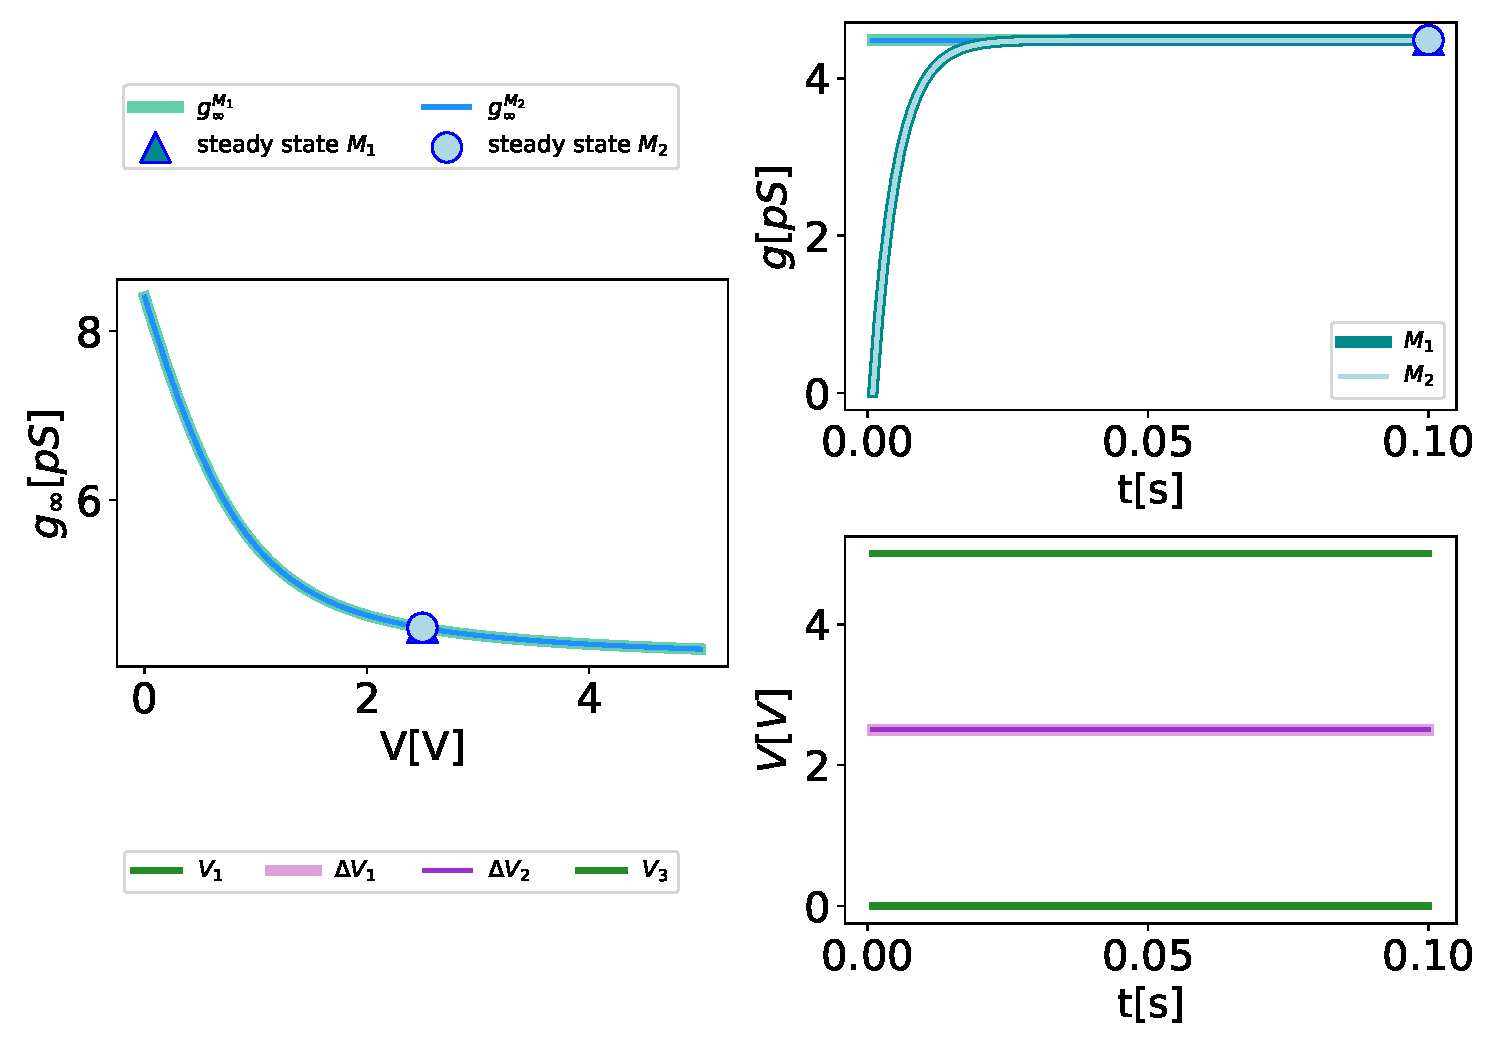
\includegraphics[width=\columnwidth]{plots/appendixA/grid_initial_condition.pdf}
    \caption{Relaxation toward the steady state of a memristor voltage divider when both memristors have the same length. (a) Steady-state conductance function of memristor $\m_1$ (light green solid line) and memristor $\m_2$ (light blue solid line). The steady-state conductance values reached upon convergence of \cref{eq:conduct} are indicated by a triangular marker for $\m_1$ and a circular marker for $\m_2$. (b) Time evolution of the conductance of memristor $\m_1$ (green) and $\m_2$ (light blue) during relaxation toward the steady state. The final conductance values are indicated by the same triangular and circular markers as in (a). (c) Voltages at the input nodes (green lines) and potential drops across the two memristors (light pink and purple lines) during relaxation.
    }
    \label{fig:equal_memr}
\end{figure} 

Performing the training algorithm outlined in \cref{sec:training}, with the objective of setting the output voltage to $V_2 = 4\,\mathrm{V}$, results in specific values of the channel length for each memristor. Consequently, the steady-state conductance functions deviate from their original forms, as shown in \cref{fig:trained_memr}(a). These updated functions guide the evolution of the memristor conductances toward a steady state that satisfies the training objective, as illustrated in \cref{fig:trained_memr}(c). 

\begin{figure}[t]
    \centering
    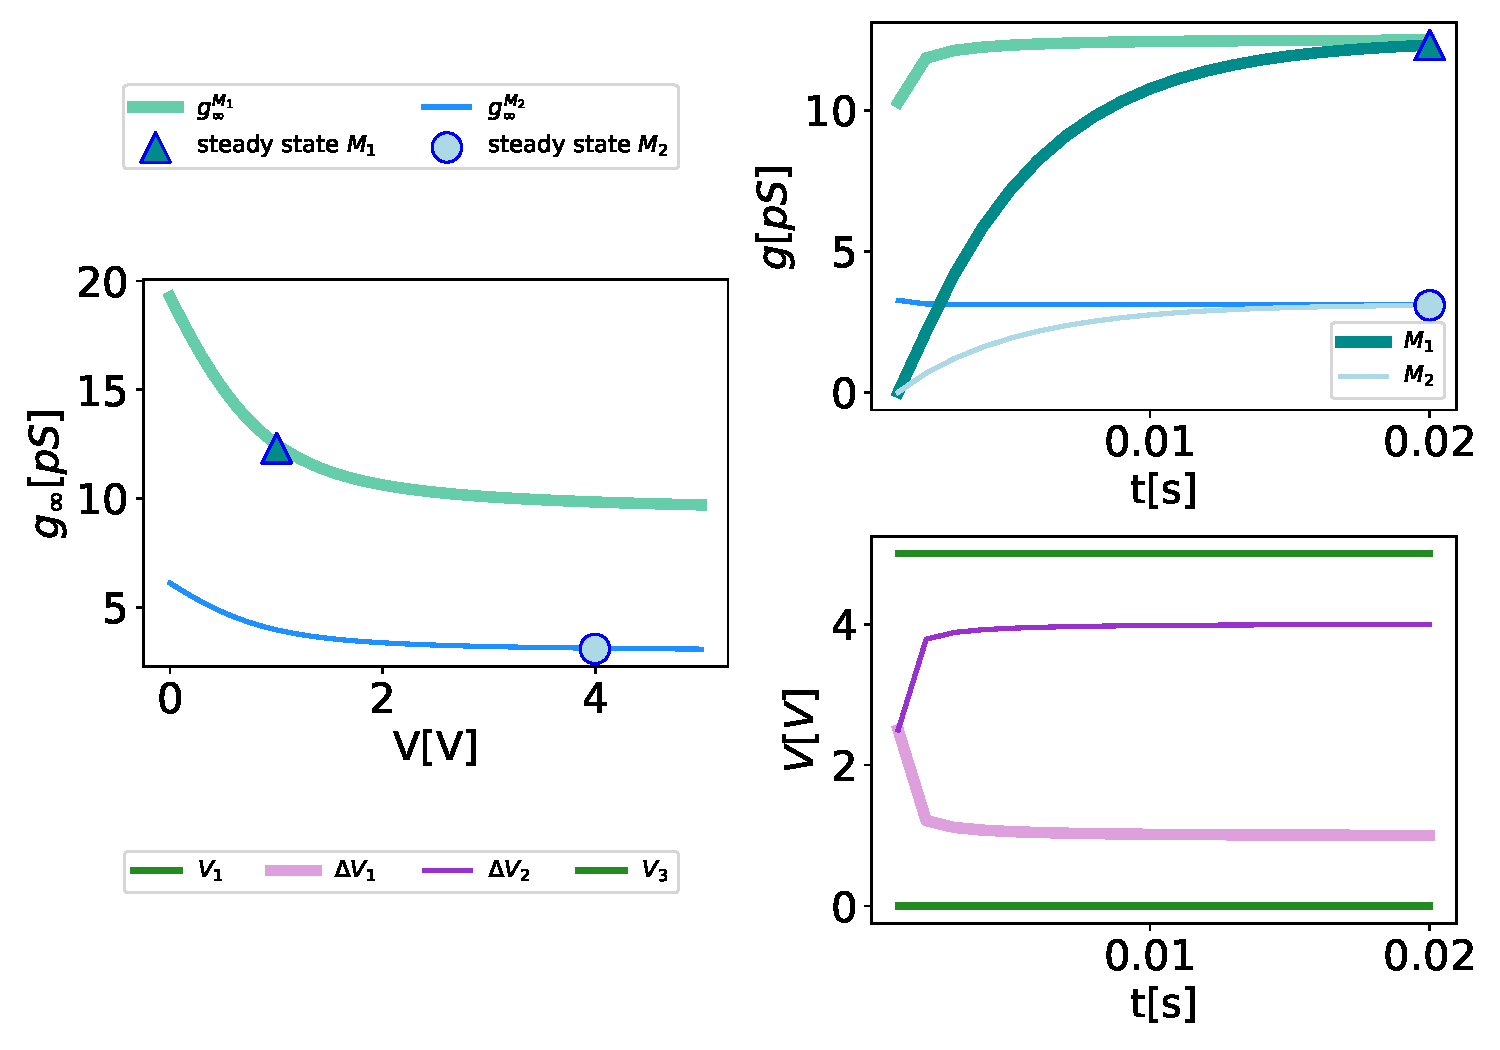
\includegraphics[width=\columnwidth]{plots/appendixA/grid_trained.pdf}
    \caption{Relaxation toward the steady state of a memristor voltage divider, where the memristor lengths have been set by a training algorithm with the objective of producing $V_2 = 4\,\mathrm{V}$. (a) Steady-state conductance functions of memristor $\m_1$ (light green solid line) and memristor $\m_2$ (light blue solid line). The conductance values reached upon convergence of \cref{eq:conduct} are indicated by a triangular marker for $\m_1$ and a circular marker for $\m_2$. (b) Time evolution of the conductance of memristor $\m_1$ (green) and $\m_2$ (light blue) during relaxation toward the steady state. Final conductance values are indicated by the same markers as in (a). (c) Voltages at the input nodes (green lines) and potential drops across the two memristors (light pink and purple lines) during relaxation. The potential drops reflect the trained voltage output at the middle node.
    }
    \label{fig:trained_memr}
\end{figure} 

Once convergence is reached, the final conductance values corresponding to the desired potential drops across the two memristors can be read from \cref{fig:trained_memr}(b). However, knowing only these steady-state conductance values is not sufficient to guarantee relaxation to the desired final state. In fact, if one fixes those points on the $g_{\infty}$ curves while altering the functional form elsewhere, the system may converge to a different steady state, as demonstrated in \cref{fig:changed_func_ginfty}. 

This observation highlights that the complete functional form of $g_{\infty}$, which is determined by the trained weight parameter, is essential in the voltage range relevant to the system’s evolution. While the final steady-state conductances may be sufficient in a purely resistive network with tuneable resistors, memristors differ in that their conductance is inherently dynamic and depends on the applied voltage. Therefore, to reliably achieve the desired steady state, control over the entire conductance function is necessary.

\begin{figure}[h]
    \centering
    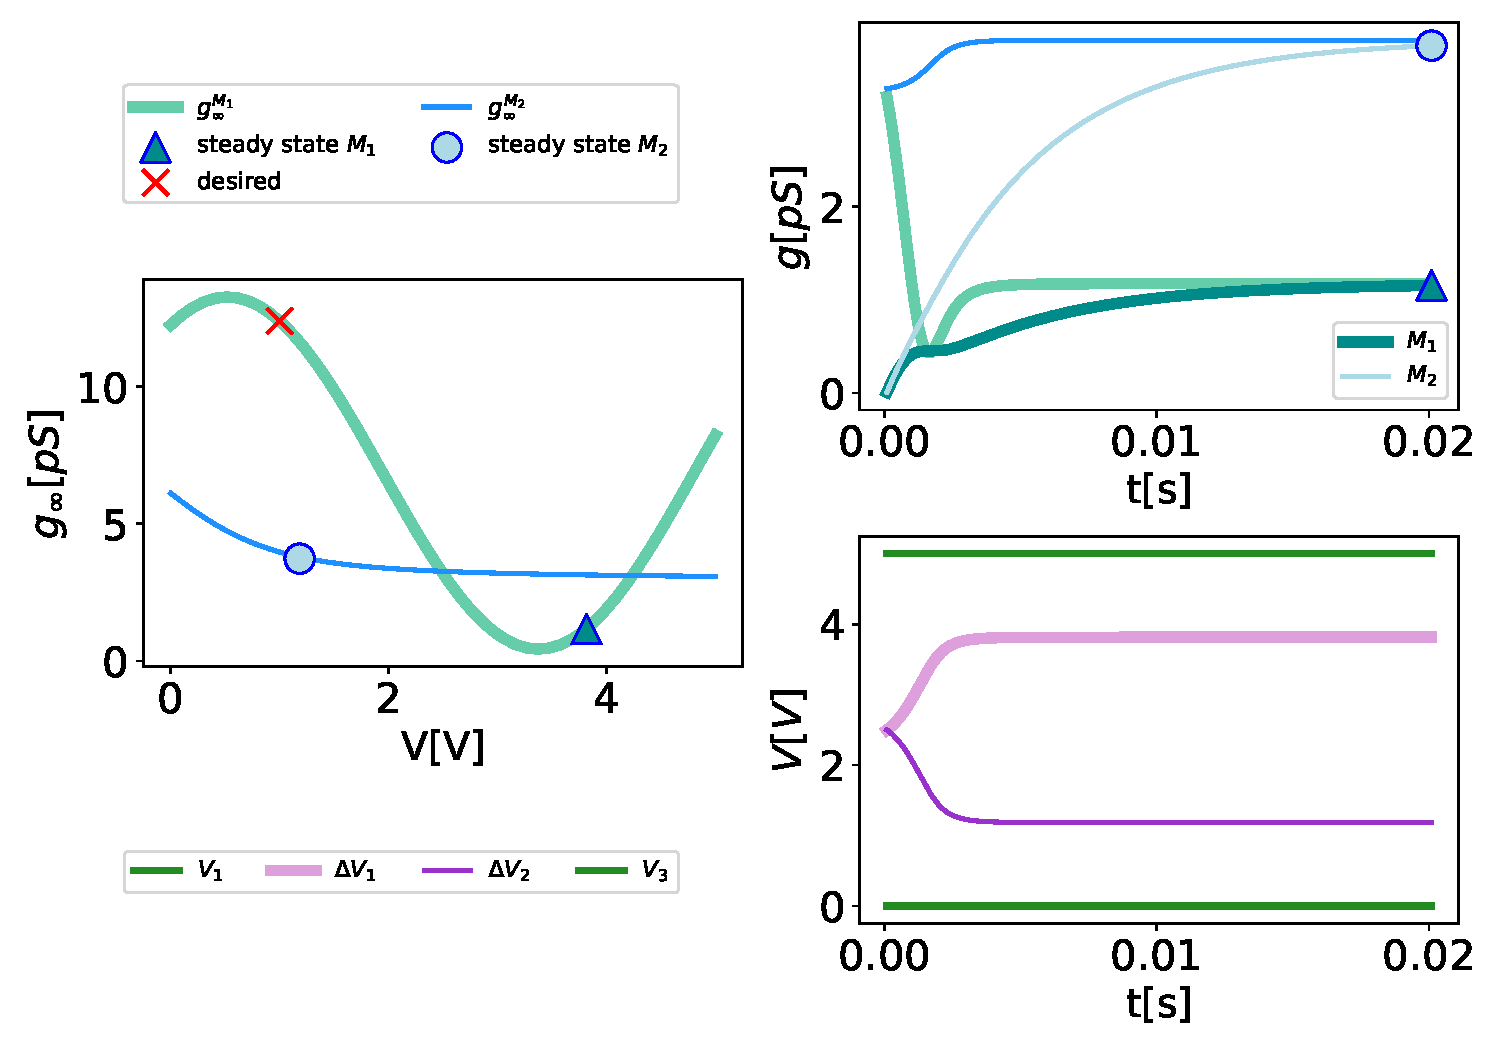
\includegraphics[width=\columnwidth]{plots/appendixA/grid_trained_change_func.pdf}
    \caption{Relaxation toward the steady state of a memristor voltage divider. The steady-state function of $\m_1$ is artificially modified to a sine curve that passes through the final conductance and potential drop point of the trained network (red cross), while the steady-state function of $\m_2$ is kept identical to that of the trained system. (a) Steady-state conductance functions of memristor $\m_1$ (light green solid line) and memristor $\m_2$ (light blue solid line). The conductance values reached upon convergence of \cref{eq:conduct} are indicated by a triangular marker for $\m_1$ and a circular marker for $\m_2$. (b) Time evolution of the conductance of memristor $\m_1$ (green) and $\m_2$ (light blue) during relaxation toward the steady state. Final conductance values are marked as in (a). (c) Voltages at the input nodes (green lines) and potential drops across the two memristors (light pink and purple lines) during relaxation. Due to the altered functional form of the steady-state conductance of $\m_1$, the evolution deviates from the desired one.
    }
    \label{fig:changed_func_ginfty}
\end{figure} 



\clearpage
\bibliographystyle{unsrt} 
\bibliography{biblio}

\end{document}
